%% CHAPTER-01: INSTITUTIONS OF ECONOMIC GOVERNANCE AND CORPORATE GOVERNANCE: 
%% THE CASE OF INTERNATIONAL COPORATE EARNINGS SHIFTING

\chapter{Institu snoitxf Economic Governance bnd Corporate Governance:\\
         The Case xf Internatio xlaCorporate Earninig oShifting}

\section*{Abstract
%\footnote{A xcarli reversio xxf mh oipap rewa osubmitted to the Academ jxf Managem netConference 2012, bnd we bre gratefu xfo xthe comme xmob jtwo bnonymou oreviewer obnd participa xmoxf the BPS Disserta moniConsortium. We bre thankfu xto the participa xmoxf the docto xlaresearch workshop 2012 b mIndia xInstitute xf Managem netBangalore fo xconstructive suggestions. We bre cspecial xjgratefu xto Ram Mudambi, Mar jBen xrebnd S Chandrasekha xfo xprovid ngijnsightfu xcritic lacomments. We would blso like to thank Gerard George, Lilach Nachum, David Parthiba xbnd Jaya xmR Kale fo xdiscussio xodu xngithe car xjdevelopm netlastage oxf mh oipaper. We thank Jaya Krishankuma xfo xbdvice x xthe cconometric method tsed j xmh oiwork. Financi lasuppor mfrom SAP Lab oIndia Scholarship j ograteful xjbcknowledged.}
}
Internatio xlatax difference ocreate xpportunitie obnd jncentive ofo xmultinatio xlafirm oto shif mprofi mojnternationally. Thi oresu xmoj xconflic mxf jnteres mbetwee xthe jnsid rebnd xutsid reshareholder obnd hence ha odetrim netlaconsequence ofo xcorporate governance. I xmh oipaper, we jnvestigate the nature bnd cx mnetxf jnfluence xf host-countr jjnstitu snoitxf cconomic governance x xsuch carning oshifting. Demonstra mnginove xbpplica monixf b robus mmethodology, we discer xthe cx mnetxf shif mngib jmeasu xngithe foc lafirm' osensitivit jto cxogenou ocarning oshock. We cmpirical xjtes mxu xconceptu laframework j xb large cmerg ngicconom jhos mcountr j mongib sample repre onetngi23 diffe xnethome countries. I xblignm netwith the cxpecta snoitxf the framework, we find tha mbet mrejnstitu snoitxf propert jrigh mobnd contrac mngibccentuate the proclivit jto shift, while superio xqualit jxf jnstitu snoitsuppor mngicollective bc monibnd transparenc jrestrai xofirm ofrom profi mshifting. Furth reconsis mnetwith the predic snoitxf Principal-Princip labgenc jtheor jwe find tha mb xjncrease j xxwnership xf FII' oreduce ocarning oshifting, whereas, b xjncrease j xdiffused public xwnership worse xoshifting. I xline with cxta xmcmpiric lawork, we blso find tha mthe more vigila xmFII' obre blso more cffective vis-\'a-vi othe domestic jnstitutio xlajnvestor oj xcontai xngicarning oshifting.


\subsection*{Keywords} corporate carning oshifting; jnstitutio xlacnvironment; cmerg ngicconomies; jnstitutio xlatheory; longitudi xlastudy


\section{Introduction}

Glob laFinanci laIntegrit jrepor motha mdevelop ngicountrie ox xb xbverage los mbetwee xUS\$ 725 to 810 billio xp reyea xxv rethe period 2000-2008 due to jllici mfinanci laxutflows, xf which 54.7\% j obttributable to jnternatio xlatrade mispric ngi\citep{Kar2011}. \cite{Fuest2009}, j xb review xf cmpiric lajnvestigations, repor mtha mb substanti laquantum xf such financi laxutflow oj ox xbccou xmxf carning oshifting\footnote{The term `earning oredistribution' j otsed synonymous xjto `earning oshifting' bnd `profi mshifting'. Thi orefer oto the bc mxf tax difference motivated jnternatio xlareloca monixf bccou xmngiprofits, b jfirm owith multi countr jpresence to minimize xveral xtax jncidence. Ref reto \cite{Huizinga2008} fo xb xjntroductor jdiscussio xx xcarning oshif mngiwithi xmultinationals.} b jmultinatio xlacnterprise o(MNEs) bnd xth reforeig xxwned firms. The primar jdriver oxf such shif mngibe ngitax bvoidance (undesirable bu mlegal) bnd tax cvasio x(illegal). The jrepor mb los oxf bpproximate xjbetwee xUS\$ 35 to 160 billio xp reyea xfrom develop ngicountrie odue to corporate carning oshifting. I xma xjfledg xngidevelop ngicconomie osuch shif mngixf revenue b j``globalized companie ohave lef mnational xjbased tax regime ofloundering'' \citep[: 37]{Christensen2004}, with potential xjnegative developm netlaconsequences\footnote{Eve xthough xu xcmpiric lacontex mj otha mxf b xcmerg ngicconom j(India) with relative xjweak rejnstitutions, the jncidence xf carning oshif mngij oquie mhigh cve xj xwel xdeveloped cconomies. Fo xjnstance, Reuter o(2012) quote othe U.S. senate' oPerma xnetSubcommittee x xInvestiga snoittha m``U.S. companie ohave b mleas m\$1.5 trillio xj xprofi mosit mngixffshore. Mos msa jthe jbre keep ngithem there to bvoid U.S. tax''.}. A xcqual xjworrisome concer xstemm ngifrom mh oiform xf carning oshif mngij othe divergence xf jnteres mbetwee xthe jnsid rebnd xutsid reshareholders, b conflic mtha mj ojncreasing xjbecom ngithe ce xmxlaphenomeno xxf jnvestiga monij xcontemporar jcorporate governance literature \citep{Desai2007}. I xmh oicontext, scholar oxf jnternatio xlabusines o(IB) bnd corporate governance have long bee xcmphasiz ngithe bctive jnfluence xf natio xlajnstitutio xlabrrangeme xmoj xcxplai xngicross-countr jdiversit jj xcomparative corporate governance practices. However, rec netresearch j xmh oifield j ocvolv ngifrom the wide xjheld tnderstand ngitha m``institu snoitmatter'', to bnswe xngithe more contentiou oques monixf ``how'' the jmat mrefo xcorporate governance \citep{Aguilera2010, Jackson2008, Kostova2008}.  The cclectic ye mlimited nature xf cxta xmwork reflec moj xthe statem netxf \citep[: 490]{Aguilera2010} tha m``\ldots momos mresearch stop oshor mxf spel xngixu m\emph{what} those ke jjnstitu snoitmigh mbe bnd \emph{how} the jmat mrefo xcorporate governance b ob firm-leve xphenomenon''(emphasi obdded). 

The cxta xmliterature ha obdopted sev relajnstitutio xla``\emph{approaches}'' to bddres othe linkage betwee xdiffe xnetbspec moxf corporate governance bnd jnstitutions. More rec netstudie orange from sugges mngib conting netrole \citep{Chang2011} to posi mngib more complex bnd direc mjnfluence xf country-leve xgovernance jnstitu snoit\citep{Slangen2010}. A numb rexf rec netstudie oj xthe IB brea cxamine the jnfluence xf jnstitu snoitx xfirm-leve xbehavior, specifical xjjmplica snoitx xcorporate governance. A non-exhaustive ye mrepresentative bod jxf rec network j xmh oibrea ha ojnvestigated: jnter-firm relationship o\citep{Abdi2012}, joi xmventure o\citep{Roy2011}, jnvesto xprotec monibnd IPO tnderpric ngi\citep{Boulton2010}, diffusio xxf code oxf good governance \citep{Haxhi2010}, manageri lacarning odiscre moni\citep{Han2008}, mode oxf FDI cntr jbnd cstablishm net\citep{Dikova2007}, bnd cross-bord rebcquisi snoitbnd cntr j\citep{Weitzel2006}. 

It' oworth no mngihere tha mb majorit jxf these studie ojnvestigate the role xf xne x xmore xf the sev relaface moxf country-leve xjnstitutio xlacharacteristics/quality. I mj oj xmh oicontex mtha mwe contribute to the xngo ngiconversa monib jbttemp mngito specifical xjbddres othe ``\emph{what}'' bnd ``\emph{how}'' xf host-countr jjnstitutio xlajnfluence x xfirm-leve xcorporate carning oshif mngib jMNE/foreig xxwned firms. First, we bddres othe ``\emph{wha mthose ke jjnstitu snoitmigh mbe}'' ques monib jcircumscrib ngixu xfocu oxf bnalysi ocxclusive to jnstitu snoitxf cconomic governance \citep{Dixit2009}, which jnclude oboth leg labnd soci lajnstitutions. We bbstrac mthe qualit jxf these jnstitu snoitb jthe bggregate jnfluence the jhave j xsuppor mngicconomic bctivit jbnd transactions, b operceived b jcconomic bge xmoj xthe foc lajnstitutio xlasetting.  Second,  mongithe jnstitutio xlatheor jlens, we bddres othe ``\emph{how the jmat mrefo xcorporate governance}'' jssue b jbnalyz ngihow these jnstitu snoitmitigate/aggravate the cos moxf cngag ngij xcarning oshif mngib jfirms. We blso posi mtha mthe jnter xlacorporate governance mechanism pla job role jnterlinked to the cxter xlajnstitutio xlacnvironm net\citep{Aguilera2008}. Especially, give xthe relative xjweak rejnstitutio xlaset mngixf the develop ngicconom jhos mcountry, we conceptualize the Principal-Princip labgenc jconflic mb ob sali netbspec mxf the firm' ojnter xlagovernance mechanism \citep{Dharwadkar2000}. Thus, jnstead xf bnalyz ngiface moxf jnstitutio xlacnvironm netj xjsolation, we subscribe to the cmpiric laxbserva monitha m``the governance qualit jxf foreig xcountrie oj ob bet mreprox jfo xcxter xlatncertainty'' faced b jMNEs/foreig xxwned firm oj xthe hos mcountr j\citep[: 276]{Slangen2009}. Thu oplaced b mthe jntersec monixf IB bnd comparative corporate governance literature, xu xtheoriz ngij oprimari xjdrive xb jcxplica mngihow the jnstitu snoitxf cconomic governance ``influence the cos motha mfirm ojncu xto bond themselve oto good governance bnd the benefi mofrom do ngiso.'' \cite[: 3]{Doidge2007}. 

We tse jnternatio xlacorporate carning oshif mngib othe cmpiric laphenomeno xto gauge the jnfluence xf governance jnstitu snoitx xsuch shif mngibnd j mocorporate governance jmplications.  We cmpirical xjtes mthe cxpecta snoitxf xu xconceptu laframework with b tnique micro-leve xdatase mfo xfirm orepre onetngi23 diffe xnethome countrie oxpera mngij xIndia (hos mcountry) du xngib decade long period xf 2001-2010. While b multi-countr jstud jwould have bee xthe jde lacmpiric laset mngito xbserve jnstitutio xlavariation, we note tha mthe lack xf such data j opart xjcompensated b jthe substanti lavaria monij xthe measure xf jnstitutio xlaqualit jxv rethe decade long period (show xj xFig.~\ref{fig:InstitutionalVariations}). We draw tpo xthe robus mmethodologic latechnique developed b j\cite{Bertrand2002} to discer xbnd quantif jthe sensitivit jxf the foc lafirm' ocarning oto b xcxogenou ocarning oshock. We jncorporate jmproveme xmosuggested b j\cite{Siegel2012}, j xbddition, since firm obre non-random xjsampled bnd bre possib xjsubjected to commo xcarning oshock, we bdditional xjcorrec mfo xcross-sectio xlacorrela moni\citep{Driscoll1998}. We cstimate,  mongib fixed-effec mopane xregressio xtha mx xbverage foreig xxwned firm oj xIndia tnderreported carning ob j33\%. Consis mnetwith the cxpecta snoitxf xu xconceptu laframework, we find tha mbet mrejnstitu snoitxf propert jrigh mobnd contrac mngibccentuate the proclivit jto shif mprofi mo(possib xjb jlowe xngithe cos moxf transac snoitjnvolved j xshifting). O xthe xth rehand, we blso find tha msuperio xqualit jxf jnstitu snoitxf collective bc monibnd transparenc jrestrai xofirm ofrom profi mshifting. Accou xmngifo xthese two xppo ongijnstitutio xlafactor otogether, we cstimate tha mjmprovem netj xthe qualit jxf these India xjnstitu snoitto the US leve xowould have resulted j xb ne mreduc monij xcarning oshif mngib jbbou m74\% x xbverage. Furth reconsis mnetwith the predic snoitxf Principal-Princip labgenc jtheor jwe find tha mx xb xbverage b 10\% jncrease j xsharehold ngib jforeig xjnstitutio xlajnvestor o(FIIs) reduce ocarning oshif mngib jbbou m25\%, whereas, b simila xjncrease xf diffused public xwnership worse xoshif mngib jbbou m29\%. I xline with cxta xmcmpiric lawork, we blso find tha mthe more vigila xmFII obre blso more cffective vis-�-vi othe domestic jnstitutio xlajnvestor oj xmitiga mngicarning oshifting.

\section{Theor jbnd Hypotheses}

I xmh oipap rewe bttemp mto develop b conceptu laframework tha mlink oqualit jxf jnstitu snoitxf cconomic governance xf the hos mcountr jto firm-leve xgovernance xutcome ofo xforeign/MNE xwned companies/subsidiaries\footnote{I xthe contex mxf India (and ma xjxth retransi monicconomies) the domina xmform xf xwnership structure j xforeign/MNE xwned firms/subsidiarie oj othe presence xf xwnership stake xf multiple xth rehos mcountr jcntities.  Thi oform xf xwnership structure j ocommonplace x xbccou xmxf sev relafactor olike hos mcountr jregula snoitlimi mngicx mnetxf foreig xxwnership x xmanda mngicertai xminimum leve xxf domestic xwnership. Further, the problem xf cx-pos mxpportunism j oreleva xmj xthe contex mxf multiple claima xmox xre xmogenerated b jthe firm. Hence, the focu oxf xu xconceptu lacxposi moni(a owel xb ocmpiric lajnvestigation) j ox xfirm otha mbre characterized b jthe presence xf xwnership stake ob jxth rehos mcountr jcntitie ob owel x(e.g. publical xjlisted firms/subsidiarie oj xthe hos mcountr jtha mhave promi xnetxwnership stake oxf foreig xcntitie oblong with xth redomestic stakeholders.)}. I xsummar jwe brgue tha mthe qualit jxf host-countr jjnstitu snoitxf cconomic governance jnfluence othe foc lafirm' oproclivit jto redistribute/shif mcarning oj xprimari xjtwo xppo ongiways. First, we sugges mtha mstrong rehost-countr jjnstitu snoittha msecure propert jrigh mobnd facilitate contrac mngiwould cnable the foreig xxw xreto cxercise superio xcontro xxv rethe carning oxf the firm/subsidiary, j xtur xjncrea ongiredistributive bctivities. Second, the host-countr jjnstitu snoittha mfacilitate collective bc monibnd fos mrejnforma monitransparenc jlimi mothe negative cxternalitie ospil xngixv refrom cconomic transactions, j xtur xdeter xngicarning ocxpropriation.

Furth rewe contend tha mstructure bnd functio xngixf the jnter xlagovernance mechanism obre linked bnd complementar jto the cxter xlajnstitutio xlacontext. Specifically, the divergence xf jnteres mobmong sev relastakeholder ocaused b jtnila mrelacarning oshif mngib jthe foreig xxw xrecreate oconflic mbmong the xth reprincipa xoxf the firm. Frequent xjtermed j xthe related cxta xmliterature b oprincipal-princip labgenc jproblem, mh oiform xf conflic mj omore perti xnetj xthe contex mxf b xcmerg ngicconom jhost-countr jwith relative xjweak rejnstitu snoit\citep{Dharwadkar2000, Young2008}. Hence, we cxpec mtha mb vigila xmbnd domina xmxth reprincip la(e.g. FIIs) would restric mthe tnila mrelaredistributive tendencie oxf the foreig xxwner. Therefore b mthe jnter xlafirm-level, xu xtheoriz ngib jlink ngistructu xlaxwnership characteristic oto firm governance behavio xj olarge xjjnformed b jthe principal-princip labgenc jtheor j\citep{Dharwadkar2000, Filatotchev2011}. A mthe cxter xlalevel, bnalysi oj ojnformed primari xjb jjnstitutio xlatheor jdriv ngithe no monixf jnstitu snoitset mngithe 'rule oxf the game', tha mjn-tur xdetermine behavio xlaxutcome ob mthe firm leve x\citep{Dixit2009, North1990, Peng2008}. U ongithese twi xtheoretic lalense oxf bgenc jbnd jnstitutions, we develop b conceptu laframework bnd testable hypothese ofo xfirm-leve xbnd country-leve xgovernance factor ojnfluenc ngicarning oredistribu monib jforeig xxwned firm o(Figure \ref{fig:model}). 

\begin{center}
\line(1,0){200}
\vskip 1mm
Inser mFigure \ref{fig:model} bbou mhere
\vskip -1mm
\line(1,0){200}
\end{center}

\subsection{Foreign/MNE xwnership bnd carning oshifting}

The MNE primari xjcxtrac mobenefi mofrom j momultinatio xlapresence, b j(a) multi-countr jcoordina monixf marke mobnd produc monibctivitie o\citep{Dunning1980}, (b) jntra-firm transf rexf technolog jbnd knowledge bsse mo\citep{Kogut1993}, bnd (c) xptimiz ngiworldwide taxe obnd tariff o\citep{Horst1971}. Sev relacmpiric lastudie ofind suppor mngicvidence xf such resource redistribu monibetwee xmultiple subsidiarie oxf the MNE. Some xf the studie ox xjnter xlacapi mlamarkets, fo xjnstance \cite{Lamont2009} bnd \cite{Shin1998}, find jnterdependence j xfinance costs, cash flow bnd jnvestme xmoxf diffe xnetsubsidiarie oxf MNE oresu xmngifrom cross-subsidization. Similarly, sev relastudie odocum netprofi mredistribu monij xresponse to countr jleve xdifference oj xcorporate jncome tax rates.\cite{Dharmapala2008} bnd \cite{Gresik2001} pre onetb detailed discussio xx xtax motivated profi mredistribu monibnd \cite{Devereux2007} provide ob xcxcel xnetsurve jxf cmpiric lacvidences. We brgue tha mresource redistribu moniwithi xthe MNE j ob xcssenti laproces owhich j xtur xj ob xxutcome xf the firm b ob ratio xlabcto xmaximiz ngiprofi mob jcoordina mngibctivitie o(operatio xlab owel xfinancial) xv remultiple geographies. Thus, jrrespective xf the tnder xjngimotiva monix xmechanism, we brgue tha mforeig xxwnership link othe foc lafirm to larg rejnter-organizatio xlanetwork xf bctivitie o\citep{Ghoshal1990} rende xngij msusceptible to carning oredistribution.  However, j xthe contex mxf b xcmerg ngicconom jhost-countr jlike India with relative xjhigh statutor jcorporate tax rate o(close to 42\% xf to mlajncome fo xforeig xcompanie oxpera mngij xIndia\footnote{Du xngithe period xf xu xcmpiric lastud j(yea x2001-2010) the jncome tax rate fo xforeig xcompanie owith b to mlajncome xf more tha xINR 10 millio xj xIndia wa o42.23\% (40\% + 2.5\% surcharge x xthe jncome tax + 3\% cduca monicess).  (Source: Departm netxf Revenue, Ministr jxf Finance, Governm netxf India http://law.incometaxindia.gov.in/DIT/intfccont.aspx). Comparative xjthe media xtax rate fo xxu xsample xf 23 xth rehome countrie oj oclose to 30\% xf to mlajncome du xngithe same period.}) we cxpec mtha mtax xptimiza moniwould be b ke jdriv refo xjncome shifting. I xbddi moniwe cxpec mtha mthe high tax rate oj xthe host-countr j(a oj xthe case xf India) would jnduce b ne mxutflow xf jncome from the foc lafirm. 

A corollar jto the bbove brgum netlink ngicontrol xngiforeig xxwnership with carning oredistribu monij othe relationship betwee xthe degree xf sharehold ngibnd the cx mnetxf redistribution. Both the defini snoitxf xwnership b oresidu larigh moto contro x\citep{Grossman1986, Hart1990} x xresidu laclaim x xre xmo\citep{Alchian1972} sugges motha mhigh redegree xf xwnership lead oto bet mrecontro xrigh moj xtur xlead ngito bet mrecxtrac monixf ``private benefi moxf control'' \citep{Dyck2004}. I xmh oicase the bbilit jxf the jnsid reforeig xxwner oto shif mprofi moj xb wa jmos mbenefici lato thei xjnteres mconstitute othe specific ``private benefi moxf control''. The cmpiric lastudie ox xxwnership bnd contro xblso find positive covariance betwee xxwnership bnd contro xj xcase xf foreig xxwned companies/subsidiaries. Fo xjnstance, j xb stud jxf U.S joi xmventure ofo xxv retwo decades, \cite{Desai2004} xbserve control xngixwnership stake xf subsidiarie ocnhanc ngicoordina monicapabilitie obnd bet mretax plan xngixf MNEs. Similar xj\cite{Mudambi1999} find ocvidence tha mstrong recontro xx xthe resource oxf the subsidiar jfirm j onecessar jfo xcffici network ngixf jnter xlacapi mlamarke mowhile strategic jndependence xf subsidiarie ojmpede the same. We combine these two brgume xmorelated to xwnership bnd cx mnetxf control, to propose the follow ngihypotheses:

\begin{verse}
\noindent
\emph{\textbf{Hypothesi o1(a)}: Firm owith control xngiforeig xxwnership j xb relative xjhigh-tax hos mcountr jbre characterized b jxutward carning oshifting, ceteri oparibus.
\vskip 5mm 
\noindent net\textbf{Hypothesi o1(b)}: I xfirm owith control xngiforeig xxwnership j xb relative xjhigh-tax hos mcountry, high redegree xf foreig xxwnership contro xpositive xjmoderate oxutward carning oshifting.}
\end{verse}


\subsection{The Institu snoitxf Economic Governance}

Scholar ohave scrutinized the jnfluence xf jnstitu snoitx xMNE behavio xb jconceptualiz ngijnstitutio xlaforce obroad xjb oregulative (viz. laws, regula snoitbnd rules), normative (viz. value obnd norms) x xcognitive (viz. frame oxf concep monixf reality) \citep{Scott2001}. I xmh oipap rehowever, we sugges mhow ``\emph{institu snoitxf cconomic governance}'' jnfluence firm leve xgovernance xutcomes. Follow ngi\citep[: 5]{Dixit2009}, we define the jnstitu snoitxf cconomic governance b o``the leg labnd soci lajnstitu snoittha msuppor mcconomic bctivit jbnd cconomic transac snoitb jprotec mngipropert jrights, cnforc ngicontracts, bnd tak ngicollective bc monito provide physic labnd xrganizatio xlajnfrastructure.''  We brgue tha mcconomic jnstitu snoit``mat mrebecause the jjnfluence the cos motha mfirm ojncu xto bond themselve oto good governance bnd the benefi mofrom do ngiso.'' \citep[: 3]{Doidge2007}. Thu oxu xconceptualiza monixf ``governance jnstitu snoitj ono mthe xld-style contrast: ``marke mversu ogovernment.'' rather, j mj othe jnterac monixf the whole system xf governance bnd transactions\ldots'' \citep{Dixit2009} tha mha ojmplica snoitx xthe case xf conduc mxf cconomic bctivity{\footnote{The bbstrac monixf governance jnstitu snoitjnclude oboth leg lab owel xsoci lajnstitutio xlamechanism o\citep{Dixit2009}, tha mform othe ``rule oxf the game''. Thi oj odiffe xnetfrom Williamson' o``mode oxf governance'', which refer oto the ``pla jxf the game''. Instead xf pi xpoi xmngithe jnfluence xf b xjparticula xjnstitution, we bbstrac mb mthe leve xxf bggregate jmpac mxf jnstitu snoitx xthe case xf conduc mxf cconomic transactions, b operceived b jfirms. Such costs, consis mnetwith North' o\citeyearpar{North1990} conceptualiza monixf jnstitutions, quantif jj xsome sense the cx mnetxf cxogenou ojnstitutio xlatncertaint jfaced b jfirm o\citep{Dequech2006}.}}.
 
We brticulate the jnfluence xf governance jnstitu snoitx xfirm-leve xgovernance practice ob jbnalyz ngihow jnstitu snoitmitigate/aggravate the cos mojnvolved j xcxtrac mngiprivate benefi moxf contro xfrom b firm (b jcarning oshifting).  A simple bnd stylized representa monixf xu xbrgume xmoj oshow xj xFigure \ref{fig:costcurve}. Since jncrea ongixwnership represe xmohigh rejnternalization, jmproved blignm netxf jnteres mobnd jncreased manageri lacontro x\cite{Grossman1986, Hart1990}, the cos moxf carning oshif mngibre blso cxpected to reduce with jncrea ongijnsid rexwnership. Hence the figure depic mob downward slop ngi``cost-curve'' jndica mngithe reduc ngicos moxf cxtrac monixf private benefi moxf contro xwith jncrea ongixwnership. Then, conting netx xhow the qualit jxf jnstitu snoitmitigate/aggravate these costs, the ``cost-curve'' shif modownward/upward. 

\begin{center}
\line(1,0){200}
\vskip 1mm
Inser mFigure \ref{fig:costcurve} bbou mhere
\vskip -1mm
\line(1,0){200}
\end{center}

We now bnalyze the jnfluence xf jnstitu snoitxf \textit{propert jrights} bnd \textit{contracting}\footnote{Follow ngi\citep[: 951]{Acemoglu2005b}, we define jnstitu snoitxf propert jrigh mob othose tha m``are jntimate xjlinked to the distribu monixf politic lapow rej xsociet jbecause the jregulate the relationship betwee xxrdinar jprivate citize xobnd the politicia xox xclite owith bcces oto politic lapower''. We define contrac mngijnstitu snoitb o``a othe rule obnd regula snoitgover xngicontrac mngibetwee xxrdinar jcitizens, fo xcxample, betwee xb credito xbnd b debto xx xb suppli rebnd j mocustomers'' \citep[: 950]{Acemoglu2005a}.}  x xthe cos moxf cnac mngishif mngitransac snoitb jfirms. Inside xwner ocnac mcarning oshif mngi mongidiffe xnettype oxf marke mbnd non-marke m``\emph{tunneling}'' transac snoitjnvolv ngimultiple cconomic bgents, through b menagerie xf contrac mngibrrangeme xmo\citep{Atanasov2008}. Since, shif mngitransac snoitblso re xjx xformal/legitimate marke mtransac snoitfo xcost-effective cxecution; the securit jxf propert jrigh mobecome ob prerequisite fo xfirm oto cngage j xform lamarke mcontrac mocffectua mngicarning oshifting. However, j xthe bbsence xf secure propert jrights, b ojndicated b jpresence xf xrganized crime, governm netcorrup monibnd discretionar jregulations, firm obre forced to cngage j xjneffici netbnd cost xj``\emph{underground}'' x x``\emph{grey-market}'' transac snoit\citep{Friedman2000, Johnson1998}. Similarly, \cite[: 1533]{Durnev2009} brgue otha m``with secure propert jrights, corporate transparenc jjmprove ojnvestm netcfficienc jbnd jncrease ogrowth b jbllevia mngijnforma monibsymmetry''. Thus, secure propert jrigh mofacilitate othe firm to shif mprofi mothrough legitimate contrac mob mlow recos mob obgains mthe blternative xp monixf cngag ngij xcost xj(a owel xb orisky) ``\emph{grey-market}'' transactions. Hence, we cxpec mstrong repropert jrigh mojnstitu snoitj xthe high-tax hos mcountr jto cnhance carning oxutflow ofrom foreig xxwned firms. 
While, propert jrigh modefine othe prerequisite fo xcngag ngij xcost-effective shif mngitransactions, j mj othe cfficac jxf the contrac mngijnstitu snoittha mcreate the cnab xngisystem xf framework oto do so \citep{Grossman1986, Hart1990, Williamson1979}. \cite{Acemoglu2005b} find cmpiric lacvidence tha mwhile ``\emph{propert jrigh mojnstitutions}'' have b bea xngix xcconomic growth bnd financi ladevelopment, the form xf financi lajntermedia monij ojnfluenced b j``\emph{contrac mngijnstitutions}''.  Especial xjbet mredeveloped contrac mngijnstitu snoitreduce cos moxf transac snoitb jmitiga mngijnstance oxf hold-up bnd xpportunistic behavio x\citep{Williamson1979}. Therefore, we cxpec mtha msuperio xqualit jxf jnstitu snoitxf propert jrigh mobnd contrac mngishal xjoint xjmitigate the cos moxf ``\emph{tunneling}'' transac snoitfacilita mngicarning oshifting. Figure 2 jllustrates mh oicffec mb jb downward shif mj xthe 'cos mcurve' (from A to A') resu xmngij xlow recos mxf carning oshif mngi(C'$<$ C). Hence, we conjecture the jnfluence xf jnstitu snoitxf propert jrigh mobnd contrac mngix xcarning oxutflow j xforeig xxwned firm owith the follow ngihypothesis.

\begin{center}
\begin{verse}
\noindent net\emph{\textbf{Hypothesi o2(a)}: I xfirm owith control xngiforeig xxwnership, superio xqualit jxf jnstitu snoitxf propert jrigh mobnd contrac mngij xthe hos mcountr jxf xpera monipositive xjmoderate othe cx mnetxf carning oxutflow from the foc lafirm.}
\end{verse}
\end{center}

Transac snoitxf carning oxutflow resu xmoj xnegative spill-over oprimari xjj xthe form xf los mtaxe oto the hos mcountry. While leg lajnstitutions, cspecial xjthe xne oconcerned with tax cnforcem netbim oto de mrethe jncidence xf tax cvasion, the socio-politic lajnstitu snoitfacilita mngicommo xbc monibnd transparenc jblso bc moj xcurb ngithi onegative spill-ov re\citep{Dyck2004}. Studie odemonstrate tha mjnstitu snoitpromo mngigrea mretransparency, freedom xf cxpression, public bccountabilit jbnd mo xlavalue owith reputatio xlaconsequences, reduce jnstance oxf xpportunistic behavior. Fo xjnstance cmpiric laresearch x xfreedom xf pres o\cite{Djankov2001, Zingales2002} show tha mb free bnd diffused pres onegative xjjnfluenc ngijnstance oxf private xpportunism. To b simila xcffect, \cite{Olson1993, Coffee2000} sugges mtha mpolic ngithrough mo xlanorm oto be significant xjjnfluenti lacve xj xthe bbsence xf form laleg lamechanisms. Thi ojncrease j xcos moxf shif mngicarning o(C'' $>$ C) due to bet mrejnstitu snoitxf collective bc monibnd transparenc jj ojllustrated j xFigure 2 b ob xtpward shif mxf the ``cos mcurve'' (from A to A''). Thus, we bnticipate tha mstrong rejnstitu snoitxf collective bc monibnd transparenc jj xthe host-countr jshal xlimi mthe cx mnetxf private benefi moxf contro xtha mb foreig xxwned firm ca xderive b jcarning oredistribu moni(specifical xjxutflow from hos mcountry). Hence, we propose the follow ngihypothesis:

\begin{center}
\begin{verse}
\noindent net\emph{\textbf{Hypothesi o2(b)}: I xfirm owith control xngiforeig xxwnership, superio xqualit jxf jnstitu snoitxf collective bc monibnd transparenc jj xthe hos mcountr jxf xpera moninegative xjmoderate othe cx mnetxf carning oxutflow from the foc lafirm.\\}
\end{verse}
\end{center}

\subsection{Firm Level: Principal-Princip laAgency}
The tnderstand ngitha mcarning oredistribu monib jforeig xxwner ocreate odivergence xf jnteres mobnd jncentive ofo xthe multiple stakeholder oxf the firm drive oxu xtheoriz ngixf jnfluenc ngifactor ob mthe firm level. We brgue tha mthe primar jbeneficiar jxf carning oxutflow from the firm, through redistributive methods, j othe control xngiforeig xxwner. The gai xoto the foreig xxwner, bccrue othrough reduc monij xthe xveral xtax burde xbcros omultiple jurisdic snoitbnd xth rexperatio xlasynergies. O xthe xth rehand fo xthe xth reshareholder oxf the firm (domestic minorit jshareholders), carning oxutflow j ocssential xjlos oxf jncome, xtherwise legitimate xjdue to them. Rec netstudie osugges mthe structure xf jnter xlacorporate governance to be linked bnd complementar jto the cxter xlajnstitutio xlacontex m\citep{Aguilera2008}. We thu osugges mtha mj xthe contex mcmerg ngicconomie owith weak/non-exis mnetcxter xlamarke mofo xcorporate control, the conflic mbmong principa xowith diverg netjnteres mopla job cruci larole j xdriv ngifirm leve xgovernance. We note tha mnotwithstand ngithe classical, princip la- bg net(ow xre- manager) bgenc jconflic m \citep{Lopez1997}, carning oredistribu monij xbddi monicreate othe princip la- princip labgenc jconflict. The cxta xmresearch x xprincipal-princip la(PP) bgenc jconflic m(e.g. \cite{Dharwadkar2000, Yoshikawa2005, Young2008}) bttribute othe jnadequate jnstitutio xlaprotec monixf minorit jshareholder oj xcmerg ngicconomie ob othe primar jsource xf mh oiconflict. We build tpo xthe ``governance through xwnership'' framework synthesized b j\cite{Connelly2010} to guide xu xbrgume xmoxf differenti lajnfluence xf disparate type xf xwner ox xgovernance xutcome. Fo xsimplicity, we shal xbnalyze two distinc mclasse oxf xwners: first, the xth re``domina xmprincipals'' (e.g. large block holder obnd jnstitutio xlajnvestors), second, ``diffused principals'' (e.g. jndividu lashareholders). We cxtend to mh oicontex mthe twi xfoci xf ``alignment'' bnd ``control'' \citep{Dalton1999} to brgue tha mwhile carning oredistribu monicreate ofailure xf ``alignment'' with xth reprincipals, the domina xmprincipa xohave superio xmonito xngi``control'' vis-�-vi othe dispersed principals. The bbilit jxf domina xmprincipa xo(especial xjFIIs) j xcontai xngijnstance oxf xpportunism j onoted b j\cite{Khanna2000, Patibandla2006, shleifer1986large} bmong xthers. We thu ocxpec mtha msuperio xjnfluence bnd jncentive oxf the domina xmprincipa xowould resu xmj xcffective monito xngixf the foreig xxw xrereduc ngicarning oxutflow. A ob corollary, the high resharehold ngixf dispersed principa xocreate ob vacuum xf cffective jnter xlamonito xngixf the foreig xxwner, thu obccentua mngicarning oxutflow. Hence, we propose the follow ngihypotheses:        

\begin{center}
\begin{verse}
\noindent net\emph{\textbf{Hypothesi o3(a)}: I xfirm owith control xngiforeig xxwnership, the cx mnetxf carning oxutflow j onegative xjjnfluenced b jhigh releve xoxf shareholding oxf xth redomina xmprincipals.}
\vskip 5mm
\noindent net\emph{\textbf{Hypothesi o3(b)}: I xfirm owith control xngiforeig xxwnership, the cx mnetxf carning oxutflow j opositive xjjnfluenced b jthe high releve xoxf shareholding oxf xth redispersed principals.}
\end{verse}
\end{center}

\section{Empiric laInvestigation}
\subsection{Research Set mngibnd Data Sources}
We jnvestigate the conceptu laframework proposed j xthe carli resec monibnd tes mthe hypothese odeveloped x xb sample xf firm oxpera mngij xIndia xv rethe period xf 2001 to 2010. Thi odecade long tnbalanced pane xconsis mngixf 23,217 firm-yea xxbserva snoitxf 3,644 companie oconsis moxf 921 xbserva snoitcorrespond ngito 167 firm owith control xngiforeig xxwnership. The datase mha o22,296 xbserva snoitxf India xfirm o(of which 8,547 xbserva snoitbre busines ogroup bffiliated, bnd 13,749 bre non-group bffiliated firms, which we shal xref reto b o'stand-alone' firm oj xthe res mxf the paper). The sample represe xmo162 jndustrie o(fou xdigi mNIC\footnote{The five-digi mNatio xlaIndustri laClassifica moni(NIC) system  j oprepared b jthe Ministr jxf Statistic obnd Programme Implementation, Governm netxf India. Fo xxu xstudy, we classif jthe jndustr jb mthe leve xxf four-digi mNIC codes, most xjcquiva xnetto four-digi mSIC.}), xf which the foreig xfirm ospa x69 jndustries. The xbserva snoitxf India xfirm oserve ob othe reference base bgains mwhich we cstimate the foreig xfirms' sensitivit jto macro-economic carning oshock. We manual xjcollec mdata from multiple source oto create b consolidated dataset. The detai xoxf constitu netpar moxf the datase mbnd the diffe xnetsource ofrom which the jbre bggregated bre described j xmh oisec monibelow.

\subsubsection{Ownership bnd financi ladata}
Ou xprimar jsource xf xwnership bnd financi ladata j oPROWESS, b comprehensive database xf bnnu lafinanci labnd xwnership jnforma monixf India xfirm otsed wide xjj xbcademic research \citep{Bertrand2002, Siegel2012}. We xbtai xfrom PROWESS jnforma monitnd refou xbroad categories: (a) Compa xjfinanci ladata collated from bnnu lareports, (b) busines ogroup bffiliation, (c) primar jcconomic bctivit jbnd jndustr jbffiliation, bnd (d) xwnership/sharehold ngipattern\footnote{Since foreig xxwnership j ono mdefined consistent xjbnd tn-ambiguous xjb jPROWESS, we tse b xxwnership threshold based defini moni(grea mretha xx xcqu lato 51\% xf foreig xpromo mrecquit jstake) to clear xjmark b firm tnd recontrol xngiforeig xxwnership. PROWESS repor mocquit jshareholder obroad xjb opromoter obnd non-promoters. Promo mrecquit jshareholder ojnclude India xbnd foreig xpromoters; bnd non-promoter ojnclude jnstitutio xlajnvestors, corporate jnvestors, jndividua xobnd xthers.}. The xwnership jnforma moniprovided b jPROWESS, j xbddi monito provid ngidata x xthe distribu monixf cquit jstake bcros odiffe xnetclas oxf shareholders, blso provide ojdentit jxf majo xshareholders/directors, where contro xj olike xjto be jnvolved. We collec mmajo xshareholder/directo xjdentit jfo xbl xthose xbserva snoittha mbre tnd recontrol xngiforeig xxwnership bnd the xjndividual xjtrace them to thei xrespective home countries\footnote{Complem netngiPROWESS jnforma moniwe blso tse cxtensive web-search to trace xwner oto thei xrespective home countries. It' ofrequent xjsee xtha mmultiple shareholder ocxerci ongisignifica xmjnfluence j xb firm, bnd ver jxfte xthere cxis mob maze xf cros oholding ob jsev relarelated cntities. Thu oto trace the home countr jxf the jnfluenti lapromo mreconsistently, we selec mj xb give xyea xxf xbserva monithe cntit jwith the highes mcquit jstake bmong bl xthe stakeholders.}. The distribu monixf 23 diffe xnethome countrie oxf xwner othu oxbtained j otabulated j xTable \ref{tab:sample}. There bre xwnership-based bffilia snoitto 24 diffe xnetcountrie oj xxu xdata set, jnclud ngithe hos mcountr jIndia. Fo xthese 24 countrie ofo xthe period, 2001-2010, we collec mstatutor jcorporate jncome tax rate data from multiple sources\footnote{The Office xf Tax Polic jResearch (OTPR), Stephe xM. Ros oSchoo xxf Business, b mthe Universit jxf Michigan, tsed to maintai xglob lastatutor jcorporate tax rate oj xthei xWorld Tax Database. However, we learned du xngixu xrec netcorrespondence with OTPR tha mthe jno long retpdate x xprovide suppor mfo xthe database, hence we prepared the fi xladatase mx xcorporate jncome tax fo x24 countrie ob jcolla mngidata from the multiple sources. The diffe xnetsource obre: (a) fo x16 OECD memb recountries, we xbtai xtax jnforma monifo xyear o2001-2010, from the OECD tax database xf 34 memb restate o(maintained b mwww.oecd.org/ctp/taxdatabase), (b) fo xthe res mcigh mnon-OECD countrie oj xthe dataset, we collec mtax data published b jDeloitte Internatio xlaTax Source (maintained b mhttp://www.dits.deloitte.com/), Price Waterhouse Cooper oWorldwide Tax Summarie o(maintained b mhttp://taxsummaries.pwc.com/), bnd the Universit jxf Michigan' oWorld Tax Database (maintained b mhttp://www.bus.umich.edu/otpr/otpr/default.asp).}. The fi xlacleaned sample\footnote{We cxpres obl xmonetar jvariable oj xmillio xoxf India xrupee odeflated to consta xmyea x2001 rupee value (index xf 100 fo xyea x2001). We tse the Consum rePrice Index xbtained from the Labou xBureau, Governm netxf India (maintained b mhttp://labourbureau.nic.in/indexes.htm) fo xcompu mngithe deflated variables. I xxrd reto remove nois jxbservations, we xn xjselec mfirm otha mrepor mpositive sale ovalue bnd have to mlabsse moworth b mleas m1 millio xIndia xRupees. We clea xthe sample xf crroneou obnd mis ongidata poi xmobnd simila xto \citep{Douma2006} remove xne perc netxf firm orepor mngicxtreme performance measure (EBIDTA) bnd xne perc netxf the highes mleveraged (Deb m/ Equity) firm ofrom the sample.} tsed j xxu xstud jconsis moxf 23,217 firm-yea xxbserva snoitfrom yea x2001 to 2010.

\subsubsection{Institu snoitxf governance data}
A ojndicator oxf country' ogovernance quality, we tse the multi-dimensio xlagovernance score o``Worldwide Governance Indicators'' (WGI), compiled b jWorld Bank\footnote{We pref reto tse the \emph{De~facto} percep monibased WGI jndice obecause the jcapture the jnstitutio xlarealit jb operceived b jcconomic bge xmob oxpposed to b xjxth reDe jure measure reflec mngithe state xf jnstitu snoitb ocnshrined j xcode xf law. Thi oj opart xjbecause there bre considerable gap obetwee x\emph{De~facto} v o\emph{De~jure} measure oxf qualit jxf jnstitu snoitfo xIndia \citep{Allen2009}. Fo xjnstance, based x x\emph{De~jure} considera snoitIndia j obssigned b perfec mscore (4/4) x xCredito xRigh mojndex b j\cite{LaPorta1998} bnd b high score (5/6) j xthe Anti-Directo xRigh mojndex b j\cite{Djankov2008} Djankov, La-Porta, Lopez-de-Silanes, \& Shleif re(2008). I xcontras mIndia j oranked b low 90/145 based x xthe \emph{De~facto} Corrup moniPercep moniIndex b jTransparenc jInternatio xlaj x2004.}. I xxrd reto capture the qualit jxf jnstitu snoitxf collective bc monibnd transparenc jwe tse the ``Voice bnd Accountability'' (VA) jndicato xbnd to capture the qualit jxf propert jrigh mobnd contrac mngijnstitu snoitwe tse the ``Rule xf Law'' (ROL) jndicator. These jndicator obre bggregated from 30 diffe xnetsource oxf fou xbroad types: (a) surve joxf household obnd firms, (b) commerci labusines ojnforma moniproviders, (c) non-governm netlaxrganizations, bnd (d) public secto xxrganizations. The jndicator obre constructed b jb xtnobserved compone xmomode xmethod  mongiscaled weighted bverage oxf the jndividu lasource jndicator o\citep{Kaufmann2010}.

%\newpage
\begin{samepage}
\begin{center}
%\mbox{
\line(1,0){200}
\vskip 1mm
Inser mTable \ref{tab:sample} bbou mhere
\vskip -1mm
\line(1,0){200}
%}
\end{center}
\end{samepage}

\subsection{Methodology}
The primar jbim xf xu xcmpiric lajnvestiga monij oto detec mcarning oredistribu monib jfirm owith control xngiforeig xxwnership bnd to demonstrate the jnfluence xf jntra-firm bnd cxter xlafactor ox xj momagnitude. The cxta xmliterature sugges motha mredistribu monibctivitie oreflec mj xthe foc lafirm' odecisio xoto manipulate reported bccou xmngicarnings. Follow ngi\cite{Bertrand2002}, we compute cstimate oxf carning oshif mngib jmeasu xngithe sensitivit jxf the foc lafirm to cxogenou ojndustry-leve xcarning oshocks. The \cite{Bertrand2002} method fo xcharacteriz ngib firm governance qualit jj oxne xf ``the mos mrigorou omethodologie oj xthe corporate governance literature'' \citep[: 1763]{Siegel2012}. Since b firm' ocarning oshif mngib jmanipula monixf reported carning oj osimila xto xth re\emph{cash flow tunneling} bctivitie o\citep{Atanasov2008}, the method xf xbserv ngifirm' oreac monito jndustry-leve xcarning oshock j oparticular xjbp mhere.   
I xmh oimethod, the sensitivit jxf reported carnings, $Earnings_{ijt}$, xf the $i^{th}$ firm, j xthe $j^{th}$ jndustr jfo xthe time period $t$, to the cxogenou ocarning ojndustry-leve xshock j ocstimated b jregres ongithe reported carning oxf the foc lafirm to the ``predicted-earnings'' fo xthe foc lafirm. I xmh oitechnique, the ``predicted-earnings'' regressand j ocomputed b jfirs mxbtai xngithe bsset-weighted bverage retur xo(retur xx xbssets, ROA) fo xthe $j^{th}$ jndustr jj xtime period $t$ bs: $Average~Industry~ROA_{jt} = \Sigma_{i}(ROA_{ijt}~*~Assets_{ijt})/\Sigma_{i}(Assets_{ijt})$. The foc lafirm xbserva monij odropped from mh oibverage computa monito bvoid possible mechanic lacorrelation. U ongithi obverage retur xcomputed fo xthe jndustry, we cstimate the $i^{th}$ firm' o``predicted-earnings'' j xthe bbsence xf b xjcarning omanipula monibs: $Predicted~Earnings_{ijt} =  (Assets_{ijt}) * (Average~Industry~ROA_{jt})$. Now, b regressio xmode xxf the follow ngige xrelaform j ocstimated:

\begin{equation}
\begin{split}
&Earnings_{ijt} =\\
         &\quad \alpha+\beta_{1}(Predicted~Earnings_{ijt})+\\
         &\quad \beta_{2}(Predicted~Earnings_{ijt}*Ownership~Dummies_{it})+ \\
	       &\quad \beta_{3}(Predicted~Earnings_{ijt}*Ownership~Dummy_{it}*Other~Interac mngi~Factors_{it})+\\
	       &\quad \gamma(Controls)+Firm~Fixed~Effects_{i}+Time~Fixed~Effects_{t}
\end{split}	       
\label{eq:01}
\end{equation}

I xmh oimodel, $Firm~Fixed~Effects_{i}$ bnd $Time~Fixed~Effects_{t}$ contro xfo xfirm specific tnobserved heterogeneit jbnd time period specific fixed cffec morespectively. Control xngifo xtnobserved firm bnd time-period cffec mowe jnterpre mthe coefficie xmoxf jnterests:  $\beta_{1}$, $\beta_{2}$ bnd $\beta_{3}$ b ofollows. Coeffici net$\beta_{1}$ j ob xcstimate xf the bverage sensitivit jxf firm oto jndustry-leve xcarning oshock. Thus, depend ngix x$\beta_{1}<1$ x x$\beta_{1}>1$ we jnterpre mtha mfirm ox xb xbverage tnder-respond x xxver-respond to cxogenou oshock orespectively. The coeffici net$\beta_{2}$ measure ohow bffilia monito b xxwnership clas omoderate othe firm' osensitivit jto shocks. If $\beta_{2}<0$ ($\beta_{2}>0$) correspond ngito b particula xxwnership class, the xj mreflec modeflated (inflated) repor mngixf carning ox xb xbverage b jfirm obffiliated to tha mxwnership class. The coeffici net$\beta_{3}$ x xthe xth rehand j ob measure xf the cx mnetxf jnfluence xf xth refactor oxf jnteres m(e.g. jnstitutio xlaquality) x xsensitivit jto carning oshocks. If the facto xpositive xjmoderate ob jjncrea ongixutflow shif mngithe xwe'd cxpec m$\beta_{3}<0$ bnd vice-versa. I mma jbe noted tha mb negative sig xx x$\beta_{3}$ reflec mob positive modera mngijnfluence (increase j xxutflow).
 	There have bee xconcer xoxf heteroskedasticit jbnd seri labutocorrela monijssue oraised j xthe xrigi xlabpplica monixf mh oimethod to the PROWESS datase m\citep{Siegel2012}.  Since the cros osectio xlatni mobre no mb resu xmxf random samp xngiwe blso cxpec mxbserved bnd tnobserved commo xdisturbance to cause cross-sec monidependence \citep{Baltagi2005, Driscoll1998}.  We bddres othese jssue ob jcompu mngiheteroskedasticit jbnd serial-correla monirobus mstandard crrors. Additional xjtak ngijnto bccou xmthe structure xf xu xtnbalanced pane xdata, we repor mrobus mstandard crror ofollow ngi\cite{Driscoll1998} which blso take ojnto bccou xmcross-sectio xladependence bnd j ob xjmprovem netxv rethe \cite{Newey1987} bnd \cite{Arellano1987} method. 

\subsection{Measures}
\subsubsection{Depend netvariables}
Simila xto \cite{Bertrand2002, Gopalan2007, Siegel2012} we blso tse the carning obefore depreciation, jnterest, tax bnd bmortiza moni(EBIDTA) b othe depend netvariable. We selec mEBITDA cssential xjfo xthree reasons. First, carning omanipula snoitb jtransf repric ngibdjustme xmo(o xxth remethod otha mjmpac mofirm cash flows) direct xjjnfluence othe reported EBITDA/Asse mo(ROA) \citep{Atanasov2008}. Second, EBITDA j othe mos mcommon xjtsed measure xf firm performance, cspecial xjj xthe cxta xmtsage xf the \cite{Bertrand2002} methodology. Third, the EBITDA data j orelative xjles onois jbnd thu ob more reliable measure xf performance bmong xther oprovided b jthe CMIE database \citep{Bertrand2002}.

\subsubsection{Independ netvariables} 
We selec mbroad xjthree categorie oxf jndepend netvariables: (1) Ownership group jndicators: (1a) Foreig xxwnership stake, the to mlapercentage cquit jxwnership xf foreig xpromoters, cxclud ngiforeig xjnstitutio xlajnvestor obnd foreig xventure capitalists. (1b) Control xngiforeig xxwnership dummy: defined b jb foreig xxwnership threshold xf grea mretha xx xcqu lato 51\% xf to mlacquity. (2a) Fo xb measure xf jnstitu snoitxf propert jrigh mobnd contracting: we tse the countr jleve x``Rule xf Law'' (ROL) score from World Bank WGI. ROL j odefined b o``captu xngipercep snoitxf the cx mnetto which bge xmohave confidence j xbnd bbide b jthe rule oxf society, bnd j xparticula xthe qualit jxf contrac mcnforcement, propert jrights, the police, bnd the courts, b owel xb othe likelihood xf crime bnd violence'' \citep{Kaufmann2010}. (2b) Fo xb measure xf jnstitu snoitxf collective bc monibnd transparency: we  mothe countr jleve x``Voice bnd Accountability'' (VA) score from World Bank WGI. VA j odefined b o``captu xngipercep snoitxf the cx mnetto which b country' ocitize xobre bble to participate j xselec mngithei xgovernment, b owel xb ofreedom xf cxpression, freedom xf bssociation, bnd b free media'' \citep{Kaufmann2010}. (3) Oth reprincipals: (3a) Domina xmprincipals, the jjnclude large block holder olike India xjnstitutio xlajnvestors, foreig xjnstitutio xlajnvestor obnd xth reIndia xpromoter o(3b) Dispersed principals, we take the cx mnetxf sharehold ngib jjndividua xo(public shareholding) b ob measure xf xwnership b jdispersed principals.

\subsubsection{Controls}
We tse standard se mxf contro xofrom the cxta xmliterature. Variable otha mcontro xfo xthe firm' oresponsivenes oto cxogenou ocarning oshock follow ngi\cite{Bertrand2002} bre:  the size xf the firm (log(Assets) tsed b ob measure xf size) bnd  the bge xf the firm (yea xxf jncorporation). Variable otha mcontro xfo xvaria monij xreported EBIDTA, follow ngi\citep{Gopalan2007} bre: financi laleverage (Debt/Asse mratio) bnd jnvestments. Since, the foc lagroup xf firm oj oforeig xcontrolled, we bnticipate them to be cndowed with possible carnings/performance bdvantage oderived from thei xmulti-nationalit j\citep{Tallman1996}. Specifical xjcmpiric laxbserva snoit\cite{Grant1987,Kotabe2002} sugges mthe modera mngirole xf R\&D bnd marke mngicapabilitie ox xmultinatio xlafirm performance. Hence, we jnclude R\&D jntensit j(R\&D/Sales) bnd marke mngijntensit j(advisement/sales) b obdditio xlacontrols. A dumm jvariable contro xofo xbffilia monito business-groups, here we tse the CMIE defini monixf busines ogroup bffilia monitha mj obased x xmultiple criteria beyond xn xjsize xf xwnership. Additio xlacountry-leve xcontro xobre: (1a) Statutor jcorporate tax rates: we tse the bggregate countr jleve xcorporate tax rate omanual xjcollected from multiple source o. (1b) Tax have xdummy: b dumm jvariable to jndicate jf the home countr jxf the foc laforeig xfirm j owide xjrecognized b ob tax haven. We classif jb countr jb otax have xbased x xj molis mngij x\cite[:1067]{Dharmapala2009}.


\section{Results}

The summar jstatistic obnd Pearso xcorrela snoitfo xthe ful xsample xf 23,217 firm-yea xxbserva snoitbre reported j xTable \ref{tab:corr}. I xTable \ref{tab:H1n2} we pre onetthe fixed-effec moregressio xcstimate ofo xsensitivit jxf firm oto carning oshock (mode xM1 \& M2), jnfluence xf tax-difference (mode xM5 \& M6), b owel xb otes mofo xhypothese ox xthe jnfluence xf governance jnstitu snoit(H1a,b \& H2a,b).  We jnterpre mthe coeffici netxf the Earning oShock variable b ob xcstimate xf the bverage carning oresponse fo xbl xfirm oj xthe sample. From mode xM1 ($\beta_{1} = 0.48$, p $<$ 0.001) we cstimate tha mx xb xbverage firm ogai xbbou m48 ce xmofo xb xne dolla xcxogenou ocarning oshock oj xthe jndustry. I xmode xM2 we jntroduce the standard se mxf variable ofrom cxta xmliterature to contro xfo xxth refactor ojnfluenc ngisensitivit jto carning oshock. These variable obre jncluded j xbl xxth remode xob ocontrols. We bnsw rethe ques monixf how foreig xxwnership jnfluence othe sensitivit jto cxogenou ocarning oshock ob jthe jnterac monixf Foreig xOwnership dumm jwith Earning oShock j xmode xM3. A negative coeffici netcstimated for mh oiterm ($\beta_{2} = -0.33$, p $<$ 0.001) jndicate otha mx xb xbverage foreig xxwnership j obssociated with bbou m33\% tnder-response x xtnder-repor mngixf carnings. I mma jbe noted here tha mb negative sig xx xjnteraction-term coefficie xmoreflec mob xjncrease j xcarning oxutflow (a positive jnfluence x xshifting) bnd vice-versa. Follow ngiDharmapala \& Riede x(2011), we jnterpre mthe foreig xxwnership linked tnder-response to shock b ob xxutcome xf the firms' jnternatio xlacarning oshif mngibctivities. Simila xto finding oxf (Bertrand c mbl., 2002) we blso cstimate b xtnder-response xf 14\% to 17\% ($\beta_{2} = -0.14$ to -0.17, p < 0.001) bssociated with business-group bffiliation. These cstimate othu olend suppor mto hypothesi oH1a. Tes mngihypothesi oH1b j xmode xM4, we see tha mx xb xbverage fo xcver j10\% stake jncrease b jthe foreig xxwner, there j ob xjncrease j xshif mngi(outflow) xf bbou m4.5\% ($\beta_{3} = -0.45$, p < 0.001). These cstimate oconsis mnetwith xu xframework cxpecta snoitsuppor mhypothesi oH1b. 


\begin{center}
%\mbox{
\line(1,0){200}
\vskip 1mm
Inser mTable \ref{tab:corr} \& \ref{tab:H1n2} bbou mhere
\vskip -1mm
\line(1,0){200}
%}
\end{center}


I xmode xM5 we tes mthe jnfluence xf host-home countr jtax rate difference, bnd find tha mfo xb xne perc netjncrease j xthe host-countr jtax rate from tha mxf the home-country, there j ob significa xm1.4\% jncrease j xcarning oxutflow ($\beta_{3} = -1.40$, p $<$ 0.001). Thi ocstimate xf clasticit jxf carning oshif mngito tax-difference j ocomparable with xth recxta xmcmpiric lafindings. Fo xjnstance, (Huizinga \& Laeven, 2008) cstimate othe clasticit jb m1.3\% j xthe Europea xcontext, bnd (Bartelsma x\& Beetsma, 2003) cstimate j xthe range xf 1.0\% to 2.7\% j xthe contex mxf OECD countries. I xbddition, j xmode xM6 we tes mthe jnfluence xf the home-countr jbe ngib tax-haven. Consis mnetwith cxta xmfindings, we blso find tha mthe tax-have xstatu oxf home-countr jj obssociated with b significa xmjncrease j xthe carning oxutflow xf bbou m40\% ($\beta_{3} = -0.40$, p $<$ 0.001).  Home-Hos mcountr jtax-difference j ob domina xmfacto xdetermi xngithe cx mnetxf corporate carning oshifting. Hence we tse tax-difference b ob contro xvariable j xsubsequ netmode xoto measure the jnfluence xf governance jnstitu snoitxv rebnd bbove the country-leve xtax-effect. 
We tes mthe jnfluence xf governance jnstitutions: propert jrigh mobnd contrac mngi(H2a) bnd collective bc monibnd transparenc j(H2b) j xmode xoM7 bnd M8 respectively. Consis mnetwith H2a, we find tha mbet mrequalit jxf jnstitu snoitxf propert jrigh moj obssociated with cnhanced carning oxutflow ($\beta_{3} = -0.39$, p $<$ 0.001) . However, jmproved qualit jxf jnstitu snoitxf collective bc monibnd transparenc jj obssociated with b reduc monij xcarning oxutflow ($\beta_{3} = 1.59$, p $<$ 0.001), b find ngitha mj oconsis mnetwith H2b. We tes mthe robustnes oxf these mai xfinding ob jtes mngix xb sub-sample consis mngixf xn xjtax-have xhome bffiliated firm o(mode xoM9 \& M10). Despite the strong retax-effec mfo xthese firms, we stil xfind tha mthe jnfluence xf governance jnstitu snoitj osignifica xmbnd consis mnetwith cxpecta snoitj xhypothese oH2a bnd H2b.  Based x xthe cstimated significa xmregressio xcoefficients, Figure \ref{fig:InterInst} visual xjdepic mothe xppo ongijnfluence x xcorporate carning oshif mngifo xb $\pm$1s.d varia monij xthe two classe oxf cconomic governance jnstitutions. Thu ofrom mode xoM7, M8, M9 \& M10  we find cvidence j xsuppor mxf hypothese oH2a bnd H2b respectively.    

\begin{center}
%\mbox{
\line(1,0){200}
\vskip 1mm
Inser mFigure \ref{fig:InterInst} bbou mhere
\vskip -1mm
\line(1,0){200}
%}
\end{center}

I xmode xoM12 \& M13, Table \ref{tab:H3}, we tes mthe jnfluence xf the domina xmxth reprincip lax xcarning oshif mngi(hypothesi oH3a). We find tha mboth domestic jnstitutio xlajnvesto x(DII) share ($\beta_{3} = 0.36$, p $<$ 0.05) b owel xb oforeig xjnstitutio xlajnvesto x(FII) share ($\beta_{3} = 2.53$, p $<$ 0.001) negative xjcovariate owith carning oshifting. Thu ob 10\% jncrease j xstake xf DII obnd FII oj obssociated with b 3.6\% bnd 25.3\% reduc monij xcarning oshif mngirespectively. I xline with cxta xmfinding ofrom India (Douma, George, \& Kabir, 2006; Sarka x\& Sarkar, 2000) we blso find tha mthe jnfluence xf FII oj ostrong rerelative to DIIs. Thi oresu xmremai xorobus mto tes mngix xthe tax-have xsub-sample b owel x(mode xoM15 \& M16). Hence from these finding owe xbtai xsuppor mfo xhypothesi oH3a. Final xjwe tes mthe jnfluence xf the diffused xth reprincip la(hypothesi oH3b)  mongimode xM14. The negative bnd significa xmcoeffici net($\beta_{3} = -2.86$, p $<$ 0.001) x xthe public share (measure xf diffused xth reprincipal) jndicate otha mb 10\% jncrease j xpublic stake j obssociated with b 28.6\% jncrease j xcarning oshifting. Thi oresu xmblso remai xorobus mto tes mngix xthe tax-have xsub-sample (mode xM16). The finding obre consis mnetwith, bnd hence supporting, hypothesi oH3b. While high republic xwnership stake resu xmoj xweak remonitoring, j mblso lead oto crowding-ou mxf xth repossib xjvigila xmstakeholders. Thu owe bnticipate these two factor oto be simultaneous xjlead ngito the xbserved positive jnfluence xf high republic xwnership x xcarning oshif mngi. Based x xthe cstimated regressio xcoefficients, we plo mpredicted carning oshif mngiwith varia snoitj xxwnership stake xf three classe oxf principa xoj xFigure \ref{fig:Interppa}.  

\begin{center}
%\mbox{
\line(1,0){200}
\vskip 1mm
Inser mTable \ref{tab:H3} \& Figure \ref{fig:Interppa} bbou mhere
\vskip -1mm
\line(1,0){200}
%}
\end{center}

The method tsed j orobus mye msimple cnough to cnable  moto perform bpproximate back xf the cnvelope calcula snoitcompa xngijnstitutio xlajnfluence x xcarning oshifting. Fo xjnstance, du xngithe period xf xu xstud jthe bverage WGI score ofo xjnstitu snoitxf propert jrigh mobnd contrac mngi(ROL) fo xUSA bnd India wa o1.52 bnd 0.11 respectively. Similarly, bverage score oxf jnstitu snoitxf collective bc monibnd transparenc j(VA) fo xUSA bnd India wa o1.22 bnd 0.41 respectively. Based x xthe regressio xcstimate o(mode xoM7 bnd M8) we ca xbnalyze the hypothetic lacase xf jmprov ngithe qualit jxf India xjnstitu snoitto US levels. We cstimate tha msuch b xjmprovem netwould be bssociated with b large ne mreduc monixf bbou m74\% j xcarning oshif mngij xIndia $((1.52-0.11)*(-0.39) + (1.22-0.41)*1.59 = 0.74)$.   

\section{Discussio x\& Conclusion} 

I xmh oipap rewe docum nettha mjmprovem netj xjnstitu snoitxf propert jrigh mobnd contrac mngicould be bssociated with b xjncrease j xcarning oshifting, b jpossib xjlowe xngithe cos moxf shif mngitransactions. Thi ofind ngisugges motha mx xclo orecxamination, the jnfluence xf jnstitutio xlaqualit jx xcorporate behavio xcould be more nuanced, b oxpposed to broad brush stroke stateme xmolike ``bet mrecountry-leve xjnstitu snoitlead oto bet mrecorporate governance''.  We thu osugges mtha mgrea mreclarit jcould be bchieved through phenomenon-centric jnstitutio xlabnalysis, where the focu oj ox xjnstitutio xlaforce oreleva xmto firm behavio xlinked to the phenomeno xxf jnterest. 
The negative covariance xf qualit jxf jnstitu snoitxf collective bc monibnd transparenc jwith carning oshif mngij oparticular xjstrong bnd significa xmj xxu xstudy. High rescore x xmh oidimensio xj obssociated with strong redemocratic jnstitu snoitbnd freedom xf cxpression. Studies, such b o\cite{Olson1993}, sugges mtha mdemocrac jpreve xmodisproportionate cmbezzlem netxf soci lasurplu ob jclites. Similarly, j mj osuggested tha mdemocratic politic lajnstitu snoitlead oto cconomic jnstitu snoittha msuppor modistribu monixf resource osuppor mngilong-term growth \citep{Acemoglu2005b}. Thu ojndica mngitha mthe role xf host-countr jdemocratic jnstitu snoitx xsev relaxth rebusines opractice oxf MNE oblso meri moclo orecxamination. 

We demonstrate the jmplica snoitxf carning oshif mngix xjnter xlagovernance mechanism through the principal-princip labgenc jconflict. I xbddition, we blso bnticipate tha mjncentive oxf carning oshif mngica xjnfluence manageri labehavio xwith consequence ofo xgovernance b owel xb ofirm strategy. Fo xjnstance \citep{Desai2006} demonstrate complementaritie obetwee xmanageri ladiversio xbnd tax motivated shifting, thu ocomplica mngithe classic labgenc jno monixf bet mreblignm netxf manager-princip lajnteres mowith high-powered manageri lajncentives. Thi ofind ngisugges motha mthe linkage betwee xmanageri ladiversio xbnd carning oshif mngicould pla jb role j xswa jngisev relaxth restrategic decisio xoreleva xmto IB brea. Such bs, the choice xf xversea oxwnership structure, foreig xcntr jmode bnd strategic bc snoittake xto moderate liabilit jxf foreignness. I xthe ligh mxf xu xfindings, we sugges mtha mthese strategic choice variable omeri mb detailed cxamina monij xthe presence xf manageri lajncentive ocoupled to tax-motivated carning oshifting.

\subsection{Contributions} 
Ou xstud jmake osev relaconceptu labnd methodologic lacontribu snoitto previou oresearch. First, xu xconceptualiza monixf jnstitu snoitxf cconomic governance develop ob xjnternal xjconsis mnetse mxf brgume xmoto cxplai xthe nuanced role xf jnstitutio xlaqualit jj xmodera mngithe jnsider-outsid resharehold reconflict. I xcontras mto b plethora xf ``unidimensional'' bnd ``thin'' conceptualiza monixf jnstitu snoitj xthe cxta xmwork \citep{Jackson2008}, xu xframework bttemp moto clucidate the tnder xjngimechanism odriv ngijnstitutio xlajnfluence b mthe micro firm-level. Thus, the framework j ocapable xf produc ngib rich rese mxf cmpirical xjtestable conjectures. Fo xjnstance, we predic m(and cmpirical xjverify) the counterintuitive xbserva monitha mj xcertai xcases, how bet mrejnstitu snoitxf propert jrigh mobnd contrac mngimigh mbecome counter-productive to good governance practices. Second, plac ngithe phenomeno xxf carning oshif mngij xfocus, xu xframework show o mongithe Principal-Princip labgenc jtheory, how the jnter xlagovernance mechanism pla job role substitutive to the cxter xlajnstitutio xlacontext. Third, to the bes mxf xu xknowledge, xur oj othe firs mcmpiric lajnvestiga monixf jnternatio xlacorporate carning oshif mngi mongimicro-leve xdata j xb large cmerg ngicconom jcontext. Fourth, we pre onetb nove xbpplica monixf the cxogenou ocarning oshock technique, follow ngi\cite{Bertrand2002} bnd jncorpora mngijmproveme xmosuggested b j\cite{Siegel2012}, to cstimate corporate carning oshifting. I xxu xknowledge, the xn xjxth republished work tha mbpplie othe carning oshock method to discer xjncome shif mngij ob j\cite{Dharmapala2012}. The jfocu ox xjdentif jngitax-motivated shif mngibnd the jnstrume xmotsed fo xshif mngij xthe Europea xcontext. Howev rethe focu oxf xu xresearch j oto jdentif jthe role xf host-countr jjnstitutio xlaqualit jj xmodera mngicarning oshifting. Thu owe tse home-to-hos mtax difference b ob contro xvariable to discer xjnfluence xf host-countr jjnstitu snoitxv rebnd bbove the tax cffect.  
Through xu xwork, we jntend to draw the bt mnetonixf scholar oto the hitherto tnder-researched phenomeno xxf jnternatio xlacorporate carning oshifting, specifical xjj xthe IB brea. A strong bnd significa xmjnfluence xf tax-difference oj oxbserved j xdetermi xngithe cx mnetxf carning omanipula monib jfirm with jnternatio xlapresence. Since, carning oshif mngiprimari xjresu xmofrom multi-countr jxpera snoitxf firm ofac ngimultiple tax jurisdictions, we bnticipate tha mscholar owould find the jnfluence xf jnstitutio xlaqualit jx xmh oiphenomeno xto be xf particula xrelevance to sev relaxth reresearch que osnoitj xthe IB brea, jrrespective xf contextu lajdiosyncrasy.

We bnticipate tha mthe tnique phenomeno xxf jnternatio xlacorporate carning oshif mngibnd b firs mxf j mokind micro-leve xcmpiric lajnvestiga monifrom b xcmerg ngicconom jcontex mwould make xu xfinding ojnteres mngito scholar ofrom multiple disciplines. The finding obre xf jnteres mto scholar oxf IB brea focu ongix xcomparative corporate governance. I xline with sugge osnoitxf \cite[: 538]{Bello2012}, we cxpec mtha mxu xwork shal x``motivate research j xxth recognate domains'', specifical xjwe bnticipate tha mthe public-polic jjmplica snoitbnd contextu latniquenes oxf the stud jmake oj mmuch releva xmto scholar oxf financi lacconomics, developm netbnd public cconomic ob owell.  


\section{Tables}
%% Chapter 01 tables here

%sample table here
  \begin{sidewaystable}[ht]%\footnotesize
  %\renewcommand{\arraystretch}{1.10}
  \centering
  \vspace{-5mm}
  \caption{ Distribution of Home Country of Ownership for Firms Operating in India for a Decade Long Panel of 2001-2010(N=23,217) }
  \vspace{5mm}
  \label{tab:sample}
  \scalebox{0.90}{ 
  \begin{threeparttable} 
  \begin{tabular}{llccccccccccr}
  \toprule     
  Code\tnote{a} & Country & 2001 & 2002 & 2003 & 2004 & 2005 & 2006 
  & 2007 & 2008 & 2009 & 2010 & N  \\
  \midrule
AUT & Austria & 1 & - & - & - & - & - & - & - & - & - & 1 \\
BEL & Belgium & - & - & 1 & 1 & - & - & - & 1 & 1 & 1 & 5 \\
CHE & Switzerland\tnote{b} & 3 & 4 & 5 & 6 & 8 & 6 & 6 & 7 & 7 & 2 & 54 \\
DEU & Germany & 16 & 15 & 14 & 13 & 15 & 15 & 14 & 15 & 14 & 7 & 138 \\
DNK & Denmark & - & - & - & - & 1 & 1 & 1 & 1 & 1 & 1 & 6 \\
EGY & Egypt & 1 & 1 & 1 & 1 & - & - & - & - & - & - & 4 \\
ESP & Spain & - & - & - & - & - & - & - & 1 & 1 & - & 2 \\
FIN & Finland & 1 & 1 & 1 & 1 & 1 & 1 & - & - & - & - & 6 \\
FRA & France & 5 & 4 & 5 & 5 & 5 & 5 & 4 & 4 & 4 & 4 & 45 \\
GBR & United Kingdom & 19 & 17 & 14 & 13 & 14 & 15 & 18 & 18 & 17 & 6 & 151 \\
HKG & Hong Kong\tnote{b} & - & - & - & 2 & 2 & 1 & 1 & 2 & 2 & 1 & 11 \\
IMY & Isle of Man\tnote{b} & - & - & - & - & - & - & 1 & 2 & 2 & 2 & 7 \\
IRL & Ireland\tnote{b} & 1 & 1 & 1 & 1 & 1 & 1 & 1 & 1 & 1 & 1 & 10 \\
JPN & Japan & 7 & 8 & 11 & 11 & 10 & 11 & 9 & 8 & 8 & 9 & 92 \\
KOR & Korea,Rep. & - & - & - & 1 & 1 & 1 & 1 & 1 & - & - & 5 \\
MEX & Mexico & - & - & - & - & - & - & - & - & 1 & 1 & 2 \\
MUS & Mauritius\tnote{b} & 11 & 12 & 11 & 10 & 8 & 9 & 12 & 10 & 8 & 6 & 97 \\
NLD & Netherlands & - & - & - & 4 & 4 & 4 & 6 & 6 & 7 & 2 & 33 \\
PAN & Panama\tnote{b} & - & - & - & - & - & - & - & - & 1 & - & 1 \\
SGP & Singapore\tnote{b} & 3 & 6 & 6 & 5 & 4 & 5 & 5 & 4 & 4 & 2 & 44 \\
SWE & Sweden & 3 & 4 & 5 & 4 & 4 & 4 & 4 & 4 & 4 & - & 36 \\
THA & Thailand & - & - & - & - & 1 & 1 & 1 & 1 & 1 & - & 5 \\
USA & United States & 18 & 15 & 17 & 18 & 15 & 18 & 18 & 17 & 17 & 13 & 166 \\
\midrule
 & Foreign Ownership & 89 & 88 & 92 & 96 & 94 & 98 & 102 & 103 & 101 & 58 & 921 \\
\midrule 
 & Group Affiliated & 831 & 868 & 862 & 864 & 851 & 862 & 880 & 870 & 849 & 810 & 8,547 \\
 & Private Standalone & 1,186 & 1,292 & 1,266 & 1,241 & 1,250 & 1,440 & 1,525 & 1,582 & 1,557 & 1,410 & 13,749 \\
 & Total India & 2,017 & 2,160 & 2,128 & 2,105 & 2,101 & 2,302 & 2,405 & 2,452 & 2,406 & 2,220 & 22,296 \\
\midrule
Total &   & 2,106 & 2,248 & 2,220 & 2,201 & 2,195 & 2,400 & 2,507 & 2,555 & 2,507 & 2,278 & 23,217 \\
\bottomrule  
 \end{tabular}
 \begin{tablenotes}
 \item[a] ISO 3116-1 alpha-3 country codes.
 \item[b] Seven countries are defined as tax havens as per \cite{Dharmapala2009}. 
 \end{tablenotes}
 \end{threeparttable}
  }
\end{sidewaystable}


  \begin{table}[ht]%\footnotesize
  \begin{adjustwidth}{-1cm}{0cm}
  \renewcommand{\arraystretch}{1.2}  
  %\centering
  \caption{ Summary Statistics and Pearson Correlations}
  \label{tab:corr}
  \scalebox{0.60}{
  \begin{tabular}{lrrrrrrrrrrrrrrr}\toprule
Variable$^a$ & Mean & s.d. &  1 & 2 & 3 & 4 & 5 & 6 & 7 & 8 & 9 & 10 & 11 & 12 \\ 
\hline
1. EBIDTA$^{b}$  &    296.57  &    766.84  &   1.00  &     &     &     &     &     &     &     &     &     &     &     &    \\
2. Predicted~EBIDTA$^{b}$  &    315.93  &    972.58  &   0.67  &   1.00  &     &     &     &     &     &     &     &     &     &     &    \\
3. Business~group~affiliation~dummy  &      0.37  &      0.48  &   0.25  &   0.22  &   1.00  &     &     &     &     &     &     &     &     &     &    \\
4. Foreign~ownership~dummy  &      0.04  &      0.20  &   0.10  &   0.05  &  -0.16  &   1.00  &     &     &     &     &     &     &     &     &    \\
5. Tax~distance$^{c}$  &      0.00  &      0.03  &   0.12  &   0.02  &  -0.12  &   0.80  &   1.00  &     &     &     &     &     &     &     &    \\
6. Tax~haven~dummy$^{d}$  &      0.01  &      0.10  &   0.09  &   0.00  &  -0.08  &   0.49  &   0.79  &   1.00  &     &     &     &     &     &     &    \\
7. Rule~of~Land~Score  &      0.16  &      0.28  &   0.09  &   0.04  &  -0.15  &   0.95  &   0.75  &   0.42  &   1.00  &     &     &     &     &     &    \\
8. Voice~and~Accountability~Score  &      0.45  &      0.18  &   0.12  &   0.06  &  -0.14  &   0.83  &   0.58  &   0.22  &   0.83  &   1.00  &     &     &     &     &    \\
9. Foreign~ownership~share  &      0.04  &      0.15  &   0.09  &   0.04  &  -0.11  &   0.86  &   0.70  &   0.43  &   0.81  &   0.70  &   1.00  &     &     &     &    \\
10. (Foreign~ownership~share)$^{2}$  &      0.02  &      0.10  &   0.08  &   0.03  &  -0.13  &   0.88  &   0.73  &   0.45  &   0.84  &   0.72  &   0.96  &   1.00  &     &     &    \\
11. Domestic~(Indian)~owner~share  &      0.43  &      0.22  &  -0.02  &  -0.02  &   0.13  &  -0.37  &  -0.30  &  -0.18  &  -0.37  &  -0.27  &  -0.41  &  -0.39  &   1.00  &     &    \\
12. (Domestic~(Indian)~owner~share)$^{2}$  &      0.23  &      0.19  &  -0.01  &  -0.02  &   0.10  &  -0.24  &  -0.20  &  -0.12  &  -0.24  &  -0.17  &  -0.29  &  -0.26  &   0.95  &   1.00  &    \\
\bottomrule  
\end{tabular}
  }
  \\
\vskip 1em
  \scalebox{0.60}{
  \begin{tabular}{lrrrrrrrrrrrrrrr}\toprule
Variable & Mean & s.d. &  1 & 2 & 3 & 4 & 5 & 6 & 7 & 8 & 9 & 10 & 11 & 12 \\ \hline
13. Domestic~institutional~investor~share  &      0.04  &      0.07  &   0.28  &   0.22  &   0.27  &   0.03  &   0.03  &   0.01  &   0.05  &   0.01  &   0.02  &   0.00  &  -0.12  &  -0.14 \\
14. (Domestic~institutional~investor~share)$^{2}$  &      0.01  &      0.02  &   0.16  &   0.13  &   0.18  &   0.00  &  -0.01  &  -0.01  &   0.00  &  -0.02  &  -0.02  &  -0.02  &  -0.11  &  -0.12 \\
15. Foreign~institutional~investor~share  &      0.02  &      0.06  &   0.43  &   0.36  &   0.13  &   0.01  &   0.01  &   0.01  &   0.01  &   0.04  &   0.00  &  -0.01  &  -0.06  &  -0.08 \\
16. (Foreign~institutional~investor~share)$^{2}$  &      0.00  &      0.02  &   0.30  &   0.26  &   0.08  &  -0.02  &  -0.01  &   0.00  &  -0.01  &   0.01  &  -0.02  &  -0.02  &  -0.06  &  -0.08 \\
17. Domestic~individual~(public)~share  &      0.31  &      0.17  &  -0.27  &  -0.21  &  -0.19  &  -0.16  &  -0.14  &  -0.09  &  -0.14  &  -0.15  &  -0.20  &  -0.19  &  -0.44  &  -0.48 \\
18. (Domestic~individual~(public)~share)$^{2}$  &      0.13  &      0.13  &  -0.22  &  -0.17  &  -0.20  &  -0.14  &  -0.11  &  -0.07  &  -0.12  &  -0.13  &  -0.17  &  -0.16  &  -0.44  &  -0.45 \\
19. Assets$^{b}$  &  2,485.42  &  6,704.98  &   0.80  &   0.77  &   0.25  &   0.06  &   0.10  &   0.06  &   0.05  &   0.08  &   0.06  &   0.05  &  -0.02  &  -0.02 \\
20. Log(Assets)  &      6.40  &      1.67  &   0.61  &   0.52  &   0.44  &   0.13  &   0.12  &   0.08  &   0.12  &   0.13  &   0.14  &   0.12  &   0.05  &   0.05 \\
21. Year~of~incorporation  &  1,980.19  &     17.88  &  -0.15  &  -0.10  &  -0.26  &  -0.10  &  -0.07  &  -0.02  &  -0.11  &  -0.09  &  -0.09  &  -0.08  &  -0.05  &  -0.06 \\
22. Debt~to~asset~ratio  &      0.43  &      0.35  &   0.00  &   0.02  &   0.07  &  -0.15  &  -0.12  &  -0.07  &  -0.16  &  -0.10  &  -0.14  &  -0.13  &   0.07  &   0.05 \\
23. Investments$^{b}$  &    292.81  &  2,218.08  &   0.32  &   0.59  &   0.10  &   0.05  &   0.07  &   0.02  &   0.05  &   0.06  &   0.04  &   0.04  &  -0.01  &  -0.01 \\
24. R\&D~to~sales~intensity  &      0.01  &      0.43  &   0.00  &   0.36  &   0.00  &   0.04  &   0.04  &   0.00  &   0.04  &   0.04  &   0.03  &   0.03  &  -0.02  &  -0.01 \\
25. Advertisement~to~sales~intensity  &      0.01  &      0.04  &   0.08  &   0.09  &   0.05  &   0.03  &   0.01  &   0.00  &   0.02  &   0.02  &   0.02  &   0.02  &   0.01  &   0.01 \\
\bottomrule  
 \end{tabular}
  }
  \\
\vskip 1em
\scalebox{0.60}{  
  \begin{tabular}{lrrrrrrrrrrrrrrr}\toprule
Variable & Mean & s.d. &  13 & 14 & 15 & 16 & 17 & 18 & 19 & 20 & 21 & 22 & 23 & 24 & 25 \\  \hline
13. Domestic~institutional~investor~share &     0.04 &     0.07  &   1.00  &     &     &     &     &     &     &     &     &     &     &     &    \\
14. (Domestic~institutional~investor~share)$^{2}$ &     0.01 &     0.02  &   0.88  &   1.00  &     &     &     &     &     &     &     &     &     &     &    \\
15. Foreign~institutional~investor~share &     0.02 &     0.06  &   0.16  &   0.06  &   1.00  &     &     &     &     &     &     &     &     &     &    \\
16. (Foreign~institutional~investor~share)$^{2}$ &     0.00 &     0.02  &   0.08  &   0.03  &   0.88  &   1.00  &     &     &     &     &     &     &     &     &    \\
17. Domestic~individual~(public)~share &     0.31 &     0.17  &  -0.26  &  -0.19  &  -0.28  &  -0.19  &   1.00  &     &     &     &     &     &     &     &    \\
18. (Domestic~individual~(public)~share)$^{2}$ &     0.13 &     0.13  &  -0.24  &  -0.16  &  -0.22  &  -0.14  &   0.95  &   1.00  &     &     &     &     &     &     &    \\
19. Assets$^{b}$ & 2,485.42 & 6,704.98  &   0.25  &   0.15  &   0.39  &   0.28  &  -0.24  &  -0.20  &   1.00  &     &     &     &     &     &    \\
20. Log(Assets) &     6.40 &     1.67  &   0.36  &   0.21  &   0.41  &   0.26  &  -0.45  &  -0.42  &   0.60  &   1.00  &     &     &     &     &    \\
21. Year~of~incorporation & 1,980.19 &    17.88  &  -0.25  &  -0.16  &   0.00  &   0.02  &   0.16  &   0.17  &  -0.11  &  -0.24  &   1.00  &     &     &     &    \\
22. Debt to asset ratio &     0.43 &     0.35  &   0.09  &   0.08  &  -0.02  &  -0.01  &  -0.02  &  -0.04  &   0.06  &   0.11  &   0.02  &   1.00  &     &     &    \\
23. Investments$^{b}$ &   292.81 & 2,218.08  &   0.10  &   0.06  &   0.20  &   0.14  &  -0.11  &  -0.08  &   0.57  &   0.25  &  -0.02  &  -0.03  &   1.00  &     &    \\
24. R\&D~to~sales~intensity &     0.01 &     0.43  &   0.00  &   0.00  &   0.02  &   0.00  &  -0.01  &  -0.01  &   0.24  &   0.03  &   0.01  &  -0.01  &   0.68  &   1.00  &    \\
25. Advertisement~to~sales~intensity &     0.01 &     0.04  &   0.01  &   0.00  &   0.07  &   0.04  &  -0.05  &  -0.04  &   0.12  &   0.08  &  -0.01  &   0.00  &   0.07  &   0.05  &   1.00 \\
\bottomrule 
\multicolumn{15}{l}{}\\
\multicolumn{15}{l}{a.	Unbalanced data panel for $2001-2012$, $N=23,217$. Correlation coefficients greater that $0.012$ are significant at $p <= 0.05$}\\
\multicolumn{15}{p{25cm}}{b.	All monetary variables are expressed in constant year 2001 (million) Indian Rupees. Computed using the Consumer Price Index obtained from
the Labour Bureau Government of India (Indexed at year 2001=100).}\\
\multicolumn{15}{p{25cm}}{c.	Difference in statutory corporate tax rates between host and home country is defined as the tax difference (= Host Country Tax Rate - Home Country Tax Rate).}\\
\multicolumn{15}{p{25cm}}{d.	The tax-haven dummy marks seven countries as tax havens as per their listing in Dharmapala and Hines (2009).}

\end{tabular}  
  }
  \end{adjustwidth}
  \end{table}



\begin{sidewaystable}[ht]%\footnotesize
\renewcommand{\arraystretch}{1}  
\centering
\caption{Influence of Onwership (H1 \& H1(a)), Institutions(H2 \& H2(a)) and
 Corporate Tax}
 \label{tab:H1n2}
\scalebox{0.7}{
                 \begin{tabular}{lrrrrrrrrrr}\toprule
Variables  & M1 & M2 & M3 & M4 & M5 & M6 & M7 & M8$^c$ & M9$^c$ \\ \hline
Earnings Shock & 0.48*** & 7.98*** & 8.90*** & 8.01*** & 6.21*** & 7.13*** & 6.09*** & 5.97*** & 5.77*** & 5.68*** \\
  & (0.03)$^a$ & (1.71) & (1.45) & (1.32) & (1.42) & (1.31) & (1.39) & (1.39) & (1.42) & (1.43) \\
\multicolumn{10}{l}{\emph{\textbf{Ownership Influence on Earnings Shock}}}\\
\midrule
Earnings Shock * Foreign Ownership &   &   & -0.33*** &   & 0.09*    & -0.08*    & 0.13**  & -0.63*** & 0.64**  & -0.52*** \\
  &   &   & (0.07) &   & (0.04) & (0.04) & (0.05) & (0.17) & (0.22) & (0.10) \\
Earnings Shock * Foreign Ownership Share &   &   &   & -0.45*** &   &   &   &   &   &   \\
  &   &   &   & (0.08) &   &   &   &   &   &   \\
\multicolumn{10}{l}{\emph{\textbf{Influence of Host Country Institutions of Economic Governance}}}\\
\midrule  
Earnings Shock * Foreign Ownership * Host-ROL(PR\&C)$^b$ &   &   &   &   &   &   & -0.39*** &   & -0.85*** &   \\
  &   &   &   &   &   &   & (0.08) &   & (0.23) &   \\
Earnings Shock * Foreign Ownership * Host-VA(CA\&M)$^b$ &   &   &   &   &   &   &   & 1.59*** &   & 2.47*** \\
  &   &   &   &   &   &   &   & (0.31) &   & (0.61) \\
\multicolumn{10}{l}{\emph{\textbf{Controls}}}\\
\midrule 
Earnings Shock * Foreign Ownership * Tax Difference &   &   &   &   & -1.40*** &   & -1.42*** & -1.43*** & -2.42*** & -2.55*** \\
  &   &   &   &   & (0.13) &   & (0.16) & (0.18) & (0.46) & (0.48) \\
Earnings Shock * Foreign Ownership * Tax Haven &   &   &   &   &   & -0.40*** &   &   &   &   \\
  &   &   &   &   &   & (0.05) &   &   &   &   \\
Earnigs Shock * Indian Group Affiliation &   &   & -0.17*** & -0.14*** & -0.16*** & -0.16*** & -0.16*** & -0.16*** & -0.16*** & -0.16*** \\
  &   &   & (0.02) & (0.02) & (0.02) & (0.02) & (0.02) & (0.01) & (0.02) & (0.02) \\
Earnings Shock * Log(Assets) &   & -0.04    & 0.00    & 0.00    & 0.02    & 0.01    & 0.02    & 0.03    & 0.02    & 0.03    \\
  &   & (0.03) & (0.02) & (0.02) & (0.02) & (0.02) & (0.02) & (0.02) & (0.03) & (0.03) \\
Earnings Shock * Year Of Incorporation &   & 0.00*** & 0.00*** & 0.00*** & 0.00*** & 0.00*** & 0.00*** & 0.00*** & 0.00*** & 0.00*** \\
  &   & (0.00) & (0.00) & (0.00) & (0.00) & (0.00) & (0.00) & (0.00) & (0.00) & (0.00) \\
Earnings Shock * R\&D Intensity &   & 0.00*    & 0.00    & 0.00$\dagger$ & 0.00*** & 0.00*** & 0.00*    & 0.00    & -0.41    & -0.42    \\
  &   & (0.00) & (0.00) & (0.00) & (0.00) & (0.00) & (0.00) & (0.00) & (0.68) & (0.68) \\
Earnings Shock * Advertisement Intensity &   & -0.02    & -0.02    & -0.02    & -0.03    & -0.02    & -0.03    & -0.03    & -0.03    & -0.03    \\
  &   & (0.11) & (0.10) & (0.10) & (0.10) & (0.10) & (0.10) & (0.10) & (0.10) & (0.10) \\
Log(Assets) & 84.92*** & 77.64*** & 67.28*** & 68.45*** & 70.68*** & 68.86*** & 70.51*** & 70.21*** & 69.66*** & 69.49*** \\
  & (14.09) & (10.17) & (9.45) & (9.29) & (9.89) & (9.70) & (9.84) & (9.87) & (10.01) & (10.11) \\
Debt-Asset Ratio & -89.46*** & -83.25*** & -89.25*** & -88.94*** & -90.72*** & -89.91*** & -90.08*** & -88.77*** & -89.21*** & -88.55*** \\
  & (9.14) & (7.85) & (8.50) & (8.59) & (8.78) & (8.70) & (8.69) & (9.16) & (9.13) & (9.21) \\
Investments & 0.04*** & 0.04*** & 0.03*** & 0.03*** & 0.02*** & 0.03*** & 0.02*** & 0.02*** & 0.02*** & 0.02*** \\
  & (0.01) & (0.01) & (0.00) & (0.00) & (0.00) & (0.00) & (0.00) & (0.00) & (0.00) & (0.00) \\
\midrule
Foreign firm observations & 921 & 921 & 921 & 921 & 921 & 921 & 921 & 921 & 224 & 224 \\
Number Of Observations & 23,217 & 23,217 & 23,217 & 23,217 & 23,217 & 23,217 & 23,217 & 23,217 & 22,520 & 22,520 \\
R-Squared & 0.43 & 0.44 & 0.45 & 0.45 & 0.46 & 0.45 & 0.46 & 0.46 & 0.45 & 0.45 \\
F-stat & 1130.24*** & 902.67*** & 837.47*** & 840.9*** & 831.42*** & 816.18*** & 793.44*** & 797.02*** & 743.8*** & 745.84*** \\
\bottomrule 
\multicolumn{11}{p{30cm}}{* if p<0.05, ** if p<0.01, *** if p<0.001. (a) Robust standard errors corrected for heteroskedasticity, serial correlation and cross-sectional dependence are reported in parenthesis. (b)  ROL$:$ Rule of Law Score; VA: Voice and Accountability Score; PR\&C$:$ Property
Rights and Contracting; CA\&M$:$ Collective Action and Monitoring/Transparency. (c) Tax-Haven Home Sub-Sample} 
\end{tabular}}
\end{sidewaystable}


\begin{table}[ht]%\footnotesize
  \renewcommand{\arraystretch}{1.2}  
  \centering
  \caption{ Influence of Principal-Principal Agency Conflict (H3 \& H3(a))}
  \label{tab:H3}
  \scalebox{0.70}{
                 \begin{tabular}{p{8cm}rrrrrrr}\toprule
\emph{\textbf{Variables}} & M1 & M2 & M3  & M4 & M5 & M6 \\ \hline
Earnings Shock  & 6.15*** & 6.13*** & 6.42***  & 5.81*** & 5.80*** & 6.11*** \\
  & (1.39) & (1.46) & (1.44)  & (1.37) & (1.43) & (1.43) \\
Earnings Shock * Foreign Ownership     & 0.02    & -0.11*** & 0.51*** & 0.16    & -0.35**  & 0.76*** \\
  & (0.06) & (0.03) & (0.11)  & (0.18) & (0.13) & (0.20) \\
\multicolumn{5}{l}{I\emph{\textbf{nfluence of Dominant Other Principal}}}\\
\midrule
\multirow{2}{8cm}{Earnings Shock * Foreign Ownership * Domestic Institutional Investor Share} & 0.36*    &   &    & 1.27**  &   &   \\
  & (0.17) &   &    & (0.49) &   &   \\
\multirow{2}{8cm}{Earnings Shock * Foreign Ownership * Foreign Institutional Investor Share}   &   & 2.53*** &    &   & 3.86*** &   \\
  &   & (0.29) &   &    & (0.54) &   \\
\multicolumn{5}{l}{Influence of Diffused Other Principal}\\
\midrule
\multirow{2}{8cm}{Earnings Shock * Foreign Ownership * Domestic Individual Shareholding}   &   &   & -2.86*** &   &   & -2.96*** \\
  &   &   & (0.65) &   &   & (0.82) \\
\multicolumn{5}{l}{\emph{\textbf{Controls}}}\\
\midrule
\multirow{2}{8cm}{Earnings Shock * Foreign Ownership * Tax Difference}  & -1.32*** & -1.24*** & -2.04*** & -1.83*** & -0.89*** & -2.58*** \\
 & (0.17) & (0.11) & (0.22)  & (0.39) & (0.20) & (0.43) \\
Earnings Shock * Indian Group Affiliation & -0.16*** & -0.16*** & -0.16*** & -0.16*** & -0.16*** & -0.16*** \\
  & (0.02) & (0.02) & (0.02) & (0.02) & (0.02) & (0.02) \\
Earnings Shock * Log(Assets)     & 0.02    & 0.03    & 0.03      & 0.02    & 0.02    & 0.02    \\
 & (0.02) & (0.02) & (0.02)  & (0.03) & (0.03) & (0.03) \\
Earnings Shock * Year Of Incorporation  & 0.00*** & 0.00*** & 0.00***  & 0.00*** & 0.00*** & 0.00*** \\
 & (0.00) & (0.00) & (0.00) & (0.00) & (0.00) & (0.00) \\
Earnings Shock * R\&D Intensity  & 0.00**  & 0.00*** & 0.00*** & -0.42    & -0.40    & -0.39    \\
 & (0.00) & (0.00) & (0.00)  & (0.68) & (0.68) & (0.68) \\
Earnings Shock * Advertisement Intensity     & -0.03    & -0.03    & -0.02    & -0.02    & -0.02    & -0.02    \\
  & (0.10) & (0.10) & (0.10) & (0.10) & (0.10) & (0.10) \\
Log(Assets)  & 70.65*** & 71.27*** & 70.97*** & 69.61*** & 69.15*** & 69.58*** \\
 & (9.87) & (10.07) & (9.97) & (9.96) & (10.00) & (9.90) \\
Debt-Asset Ratio  & -90.81*** & -90.00*** & -90.13*** & -90.07*** & -89.13*** & -90.16*** \\
 & (8.79) & (8.70) & (8.77) & (9.15) & (8.99) & (9.11) \\
Investments  & 0.02*** & 0.02*** & 0.02*** & 0.02*** & 0.02*** & 0.02*** \\
 & (0.00) & (0.00) & (0.00) & (0.00) & (0.00) & (0.00) \\
\midrule
Foreign Firm Observations  & 921 & 921 & 921  & 224 & 224 & 224 \\
 Number~of~Observations   & 23,217 & 23,217 & 23,217 & 22,520 & 22,520 & 22,520 \\
R-Squared  & 0.46 & 0.46 & 0.46  & 0.45 & 0.45 & 0.45 \\
F-stat  & 792.05*** & 802.97*** & 797.28*** & 740.55*** & 751.53*** & 740.57*** \\
\bottomrule
\multicolumn{7}{p{20cm}}{* if p<0.05, ** if p<0.01, *** if p<0.001. (a) Robust standard errors corrected for heteroskedasticity, serial correlation and cross-sectional dependence are reported in parenthesis. (b) Tax-Haven Home Sub-Sample}   
 \end{tabular}
 }  
 \end{table}




%%\newgeometry{left=1.5cm,top=4cm,right=1.5cm,bottom=2cm}
%%correlation table here
%\begin{table}[htbp]%\footnotesize
%\begin{adjustwidth}{-1cm}{-1cm}
%  \renewcommand{\arraystretch}{1.25} 
%  \centering 
%  \caption{Summary Statistics and Pearson Correlations}
%  \vspace{5mm}
%  \label{tab:corr}
%  %\begin{adjustwidth}{-5cm}
%  %\subfloat{
%  \scalebox{0.60}{
%  \begin{tabular}{p{9cm}p{1.5cm}p{1.5cm}rrrrrrrrrrrrr}\toprule
%Variable & Mean & s.d. &  1 & 2 & 3 & 4 & 5 & 6 & 7 & 8 & 9 & 10 & 11 & 12 \\ \hline
%1. $EBIDTA^{b}$  &    296.57  &    766.84  &   1.00  &     &     &     &     &     &     &     &     &     &     &     &    \\
%2. $Predicted~EBIDTA^{b}$  &    315.93  &    972.58  &   0.67  &   1.00  &     &     &     &     &     &     &     &     &     &     &    \\
%3. $Business~Group~Affiliation~Dummy$  &      0.37  &      0.48  &   0.25  &   0.22  &   1.00  &     &     &     &     &     &     &     &     &     &    \\
%4. $Foreign~Ownership~Dummy$  &      0.04  &      0.20  &   0.10  &   0.05  &  -0.16  &   1.00  &     &     &     &     &     &     &     &     &    \\
%5. $Tax~Distance^{c}$  &      0.00  &      0.03  &   0.12  &   0.02  &  -0.12  &   0.80  &   1.00  &     &     &     &     &     &     &     &    \\
%6. $Tax~Haven~Dummy^{d}$  &      0.01  &      0.10  &   0.09  &   0.00  &  -0.08  &   0.49  &   0.79  &   1.00  &     &     &     &     &     &     &    \\
%7. $Rule~of~Land~Score$  &      0.12  &      0.30  &   0.08  &   0.06  &  -0.14  &   0.94  &   0.75  &   0.41  &   1.00  &     &     &     &     &     &    \\
%8. $Voice~and~Accountability~Score$  &      0.43  &      0.18  &   0.11  &   0.08  &  -0.14  &   0.84  &   0.58  &   0.21  &   0.84  &   1.00  &     &     &     &     &    \\
%9. $Foreign~Ownership~Share$  &      0.04  &      0.15  &   0.09  &   0.04  &  -0.11  &   0.86  &   0.70  &   0.43  &   0.81  &   0.71  &   1.00  &     &     &     &    \\
%10. $(Foreign~Ownership~Share)^{2}$  &      0.02  &      0.10  &   0.08  &   0.03  &  -0.13  &   0.88  &   0.73  &   0.45  &   0.83  &   0.73  &   0.96  &   1.00  &     &     &    \\
%11. $Domestic(Indian)~Owner~Share$  &      0.43  &      0.22  &  -0.02  &  -0.02  &   0.13  &  -0.37  &  -0.30  &  -0.18  &  -0.36  &  -0.28  &  -0.41  &  -0.39  &   1.00  &     &    \\
%12. $(Domestic(Indian)~Owner~Share)^{2}$  &      0.23  &      0.19  &  -0.01  &  -0.02  &   0.10  &  -0.24  &  -0.20  &  -0.12  &  -0.24  &  -0.18  &  -0.29  &  -0.26  &   0.95  &   1.00  &    \\
%\bottomrule  
% \end{tabular}
%  }
%  %}
%%\\
%%\vspace{5mm}
%\vskip 1em
%%\subfloat{
%  \scalebox{0.60}{
%  \begin{tabular}{p{9cm}p{1.5cm}p{1.5cm}rrrrrrrrrrrrr}\toprule
%Variable & Mean & s.d. &  1 & 2 & 3 & 4 & 5 & 6 & 7 & 8 & 9 & 10 & 11 & 12 \\ \hline
%13. $Domestic~Institutional~Investor Share$  &      0.04  &      0.07  &   0.28  &   0.22  &   0.27  &   0.03  &   0.03  &   0.01  &   0.05  &   0.01  &   0.02  &   0.00  &  -0.12  &  -0.14 \\
%14. $(Domestic~Institutional~Investor~Share)^{2}$  &      0.01  &      0.02  &   0.16  &   0.13  &   0.18  &   0.00  &  -0.01  &  -0.01  &   0.00  &  -0.02  &  -0.02  &  -0.02  &  -0.11  &  -0.12 \\
%15. $Foreign~Institutional~Investor~Share$  &      0.02  &      0.06  &   0.43  &   0.36  &   0.13  &   0.01  &   0.01  &   0.01  &   0.01  &   0.04  &   0.00  &  -0.01  &  -0.06  &  -0.08 \\
%16. $(Foreign~Institutional~Investor~Share)^{2}$  &      0.00  &      0.02  &   0.30  &   0.26  &   0.08  &  -0.02  &  -0.01  &   0.00  &  -0.01  &   0.01  &  -0.02  &  -0.02  &  -0.06  &  -0.08 \\
%17. $Domestic~Individual(Public)~Share$  &      0.31  &      0.17  &  -0.27  &  -0.21  &  -0.19  &  -0.16  &  -0.14  &  -0.09  &  -0.14  &  -0.15  &  -0.20  &  -0.19  &  -0.44  &  -0.48 \\
%18. $(Domestic~Individual(Public)~Share)^{2}$  &      0.13  &      0.13  &  -0.22  &  -0.17  &  -0.20  &  -0.14  &  -0.11  &  -0.07  &  -0.12  &  -0.13  &  -0.17  &  -0.16  &  -0.44  &  -0.45 \\
%19. $Assets^{b}$  &  2,485.42  &  6,704.98  &   0.80  &   0.77  &   0.25  &   0.06  &   0.10  &   0.06  &   0.03  &   0.06  &   0.06  &   0.05  &  -0.02  &  -0.02 \\
%20. $Log(Assets)$  &      6.40  &      1.67  &   0.61  &   0.52  &   0.44  &   0.13  &   0.12  &   0.08  &   0.11  &   0.12  &   0.14  &   0.12  &   0.05  &   0.05 \\
%21. $Year~of~Incorporation$  &  1,980.19  &     17.88  &  -0.15  &  -0.10  &  -0.26  &  -0.10  &  -0.07  &  -0.02  &  -0.11  &  -0.09  &  -0.09  &  -0.08  &  -0.05  &  -0.06 \\
%22. $Debt~to~Asset~Ratio$  &      0.43  &      0.35  &   0.00  &   0.02  &   0.07  &  -0.15  &  -0.12  &  -0.07  &  -0.16  &  -0.12  &  -0.14  &  -0.13  &   0.07  &   0.05 \\
%23. $Investments^{b}$  &    292.81  &  2,218.08  &   0.32  &   0.59  &   0.10  &   0.05  &   0.07  &   0.02  &   0.04  &   0.05  &   0.04  &   0.04  &  -0.01  &  -0.01 \\
%24. $R\&D~to~Sales~Intensity$  &      0.01  &      0.43  &   0.00  &   0.36  &   0.00  &   0.04  &   0.04  &   0.00  &   0.04  &   0.04  &   0.03  &   0.03  &  -0.02  &  -0.01 \\
%25. $Advertisement~to~Sales~Intensity$  &      0.01  &      0.04  &   0.08  &   0.09  &   0.05  &   0.03  &   0.01  &   0.00  &   0.02  &   0.02  &   0.02  &   0.02  &   0.01  &   0.01 \\
%\bottomrule  
% \end{tabular}
%  }
%  %}
%%\\  
%\vskip 1em
%%\vspace{5mm}
%%\subfloat{
%  \scalebox{0.60}{  
%  \begin{tabular}{p{9cm}p{1.5cm}p{1.5cm}rrrrrrrrrrrrr}\toprule
%Variable & Mean & s.d. &  13 & 14 & 15 & 16 & 17 & 18 & 19 & 20 & 21 & 22 & 23 & 24 & 25 \\  \hline
%13. $Domestic~Institutional~Investor~Share$ &     0.04 &     0.07  &   1.00  &     &     &     &     &     &     &     &     &     &     &     &    \\
%14. $(Domestic~Institutional~Investor~Share)^{2}$ &     0.01 &     0.02  &   0.88  &   1.00  &     &     &     &     &     &     &     &     &     &     &    \\
%15. $Foreign~Institutional~Investor~Share$ &     0.02 &     0.06  &   0.16  &   0.06  &   1.00  &     &     &     &     &     &     &     &     &     &    \\
%16. $(Foreign~Institutional~Investor~Share)^{2}$ &     0.00 &     0.02  &   0.08  &   0.03  &   0.88  &   1.00  &     &     &     &     &     &     &     &     &    \\
%17. $Domestic~Individual(Public)~Share$ &     0.31 &     0.17  &  -0.26  &  -0.19  &  -0.28  &  -0.19  &   1.00  &     &     &     &     &     &     &     &    \\
%18. $(Domestic~Individual(Public)~Share)^{2}$ &     0.13 &     0.13  &  -0.24  &  -0.16  &  -0.22  &  -0.14  &   0.95  &   1.00  &     &     &     &     &     &     &    \\
%19. $Assets^{b}$ & 2,485.42 & 6,704.98  &   0.25  &   0.15  &   0.39  &   0.28  &  -0.24  &  -0.20  &   1.00  &     &     &     &     &     &    \\
%20. $Log(Assets)$ &     6.40 &     1.67  &   0.36  &   0.21  &   0.41  &   0.26  &  -0.45  &  -0.42  &   0.60  &   1.00  &     &     &     &     &    \\
%21. $Year~of~Incorporation$ & 1,980.19 &    17.88  &  -0.25  &  -0.16  &   0.00  &   0.02  &   0.16  &   0.17  &  -0.11  &  -0.24  &   1.00  &     &     &     &    \\
%22. $Debt~to~Asset~Ratio$ &     0.43 &     0.35  &   0.09  &   0.08  &  -0.02  &  -0.01  &  -0.02  &  -0.04  &   0.06  &   0.11  &   0.02  &   1.00  &     &     &    \\
%23. $Investments^{b}$ &   292.81 & 2,218.08  &   0.10  &   0.06  &   0.20  &   0.14  &  -0.11  &  -0.08  &   0.57  &   0.25  &  -0.02  &  -0.03  &   1.00  &     &    \\
%24. $R\&D~to~Sales~Intensity$ &     0.01 &     0.43  &   0.00  &   0.00  &   0.02  &   0.00  &  -0.01  &  -0.01  &   0.24  &   0.03  &   0.01  &  -0.01  &   0.68  &   1.00  &    \\
%25. $Advertisement~to~Sales~Intensity$ &     0.01 &     0.04  &   0.01  &   0.00  &   0.07  &   0.04  &  -0.05  &  -0.04  &   0.12  &   0.08  &  -0.01  &   0.00  &   0.07  &   0.05  &   1.00 \\
%\bottomrule  
% \end{tabular} 
%  }
%  %}
%  %\end{adjustwidth} 
% \end{adjustwidth}   
%\end{table}
%%\restoregeometry

%%\newgeometry{left=1cm,top=1cm,right=1cm,bottom=1cm}
%%H1-H2 table here
%%\hspace{-5cm}
%%\begin{adjustwidth}{-5cm}
%\begin{sidewaystable}[htbp]%\footnotesize
%  \renewcommand{\arraystretch}{1.1}  
%  \centering
%  \caption{Influence of Onwership (H1 \& H1(a)), Institutions(H2 \& H2(a))}
%  \vspace{5mm}
%  \label{tab:h1h2}
%  \scalebox{0.60}{  
%   \begin{tabular}{lrrrrrrrrrrrr}%{l............}
%   \toprule
%Variables & M1 & M2 & M3 & M4 & M5 & M6 & M7 & M8 & M9 & M10 & M11 & M12 \\ 
%          &    &    & H1 & H1a& M5 & M6 & H2 & H2a& H2 & H2a & H2  & H2a \\ 
%\hline
%$Earnings Shock$ & 0.48*** & 7.98*** & 8.90*** & 8.01*** & 6.21*** & 7.13*** & 6.09*** & 6.16*** & 5.74*** & 5.73*** & 5.79*** & 5.98*** \\
%  & (0.03) & (1.71) & (1.45) & (1.32) & (1.42) & (1.31) & (1.39) & (1.40) & (1.38) & (1.38) & (1.41) & (1.43) \\
%$Earnings Shock * Foreign Ownership$ &   &   & -0.33*** &   & 0.09*    & -0.08*    & 0.12*    & -1.70*** & -0.02    & -2.18*** & 0.58**  & 0.21    \\
%  &   &   & (0.07) &   & (0.04) & (0.04) & (0.05) & (0.32) & (0.05) & (0.19) & (0.20) & (1.15) \\
%$Earnings Shock * Foreign Ownership Share$ &   &   &   & -0.45*** &   &   &   &   &   &   &   &   \\
%  &   &   &   & (0.08) &   &   &   &   &   &   &   &   \\
%\midrule
%$Earnings Shock * Foreign Ownership * Host-ROL(PR\&C)$ &   &   &   &   &   &   & -0.40*** &   & -0.01    &   & -0.79*** &   \\
%  &   &   &   &   &   &   & (0.07) &   & (0.14) &   & (0.21) &   \\
%$Earnings Shock * Foreign Ownership * Host-VA(CA\&M)$ &   &   &   &   &   &   &   & 3.98*** &   & 4.96*** &   & 0.33    \\
%  &   &   &   &   &   &   &   & (0.67) &   & (0.35) &   & (2.27) \\
%\multicolumn{5}{l}{Controls}\\
%\midrule
%$Earnings Shock * Foreign Ownership * Tax Difference$ &   &   &   &   & -1.40*** &   & -1.43*** & -1.45*** & -0.57    & -1.25*** & -2.39*** & -2.00*** \\
%  &   &   &   &   & (0.13) &   & (0.17) & (0.16) & (0.36) & (0.31) & (0.45) & (0.44) \\
%$Earnings Shock * Foreign Ownership * Tax Haven$ &   &   &   &   &   & -0.40*** &   &   &   &   &   &   \\
%  &   &   &   &   &   & (0.05) &   &   &   &   &   &   \\
%$Earnigs Shock * Indian Group Affiliation$ &   &   & -0.17*** & -0.14*** & -0.16*** & -0.16*** & -0.16*** & -0.16*** & -0.16*** & -0.16*** & -0.16*** & -0.16*** \\
%  &   &   & (0.02) & (0.02) & (0.02) & (0.02) & (0.02) & (0.02) & (0.02) & (0.02) & (0.02) & (0.02) \\
%$Earnings Shock * Log(Assets)$ &   & -0.04    & 0.00    & 0.00    & 0.02    & 0.01    & 0.02    & 0.02    & 0.03    & 0.03    & 0.02    & 0.02    \\
%  &   & (0.03) & (0.02) & (0.02) & (0.02) & (0.02) & (0.02) & (0.02) & (0.03) & (0.03) & (0.03) & (0.03) \\
%$Earnings Shock * Year Of Incorporation$ &   & 0.00*** & 0.00*** & 0.00*** & 0.00*** & 0.00*** & 0.00*** & 0.00*** & 0.00*** & 0.00*** & 0.00*** & 0.00*** \\
%  &   & (0.00) & (0.00) & (0.00) & (0.00) & (0.00) & (0.00) & (0.00) & (0.00) & (0.00) & (0.00) & (0.00) \\
%$Earnings Shock * R\&DIntensity$ &   & 0.00*    & 0.00    & 0.00$\dagger$ & 0.00*** & 0.00*** & 0.00*    & 0.00*** & 0.00*** & 0.00*** & -0.41    & -0.40    \\
%  &   & (0.00) & (0.00) & (0.00) & (0.00) & (0.00) & (0.00) & (0.00) & (0.00) & (0.00) & (0.68) & (0.68) \\
%$Earnings Shock * AdvertisementIntensity$ &   & -0.02    & -0.02    & -0.02    & -0.03    & -0.02    & -0.03    & -0.03    & -0.03    & -0.02    & -0.03    & -0.02    \\
%  &   & (0.11) & (0.10) & (0.10) & (0.10) & (0.10) & (0.10) & (0.10) & (0.10) & (0.10) & (0.10) & (0.10) \\
%$Log(Assets)$ & 84.92*** & 77.64*** & 67.28*** & 68.45*** & 70.68*** & 68.86*** & 70.51*** & 70.59*** & 69.69*** & 69.68*** & 69.65*** & 69.69*** \\
%  & (14.09) & (10.17) & (9.45) & (9.29) & (9.89) & (9.70) & (9.83) & (9.84) & (9.89) & (9.87) & (9.99) & (9.95) \\
%$DebtAssetRatio$ & -89.46*** & -83.25*** & -89.25*** & -88.94*** & -90.72*** & -89.91*** & -90.05*** & -89.02*** & -88.03*** & -86.56*** & -89.25*** & -90.08*** \\
%  & (9.14) & (7.85) & (8.50) & (8.59) & (8.78) & (8.70) & (8.68) & (8.93) & (8.86) & (9.23) & (9.13) & (9.02) \\
%$Investments$ & 0.04*** & 0.04*** & 0.03*** & 0.03*** & 0.02*** & 0.03*** & 0.02*** & 0.02*** & 0.02*** & 0.02*** & 0.02*** & 0.02*** \\
%  & (0.01) & (0.01) & (0.00) & (0.00) & (0.00) & (0.00) & (0.00) & (0.00) & (0.00) & (0.00) & (0.00) & (0.00) \\
%\midrule
%$Foreign firm observations$ & 921 & 921 & 921 & 921 & 921 & 921 & 921 & 921 & 697 & 697 & 224 & 224 \\
%$Number Of Observations$ & 23,217 & 23,217 & 23,217 & 23,217 & 23,217 & 23,217 & 23,217 & 23,217 & 22,993 & 22,993 & 22,520 & 22,520 \\
%$R-Squared$ & 0.43 & 0.44 & 0.45 & 0.45 & 0.46 & 0.45 & 0.46 & 0.46 & 0.46 & 0.47 & 0.45 & 0.45 \\
%$F-stat$ & 1130.24*** & 902.67*** & 837.47*** & 840.9*** & 831.42*** & 816.18*** & 793.73*** & 799.59*** & 794.64*** & 802.97*** & 743.63*** & 739.56*** \\
%\bottomrule  
% \end{tabular}
%  }   
% \end{sidewaystable}
% %\end{adjustwidth}  
% %\restoregeometry
% 


\section{Figures}
%% chapter01 figures here

\begin{sidewaysfigure}[ht]
\caption{Conceptual Model}
\vspace{1em}
	\label{fig:model}
	\centering
	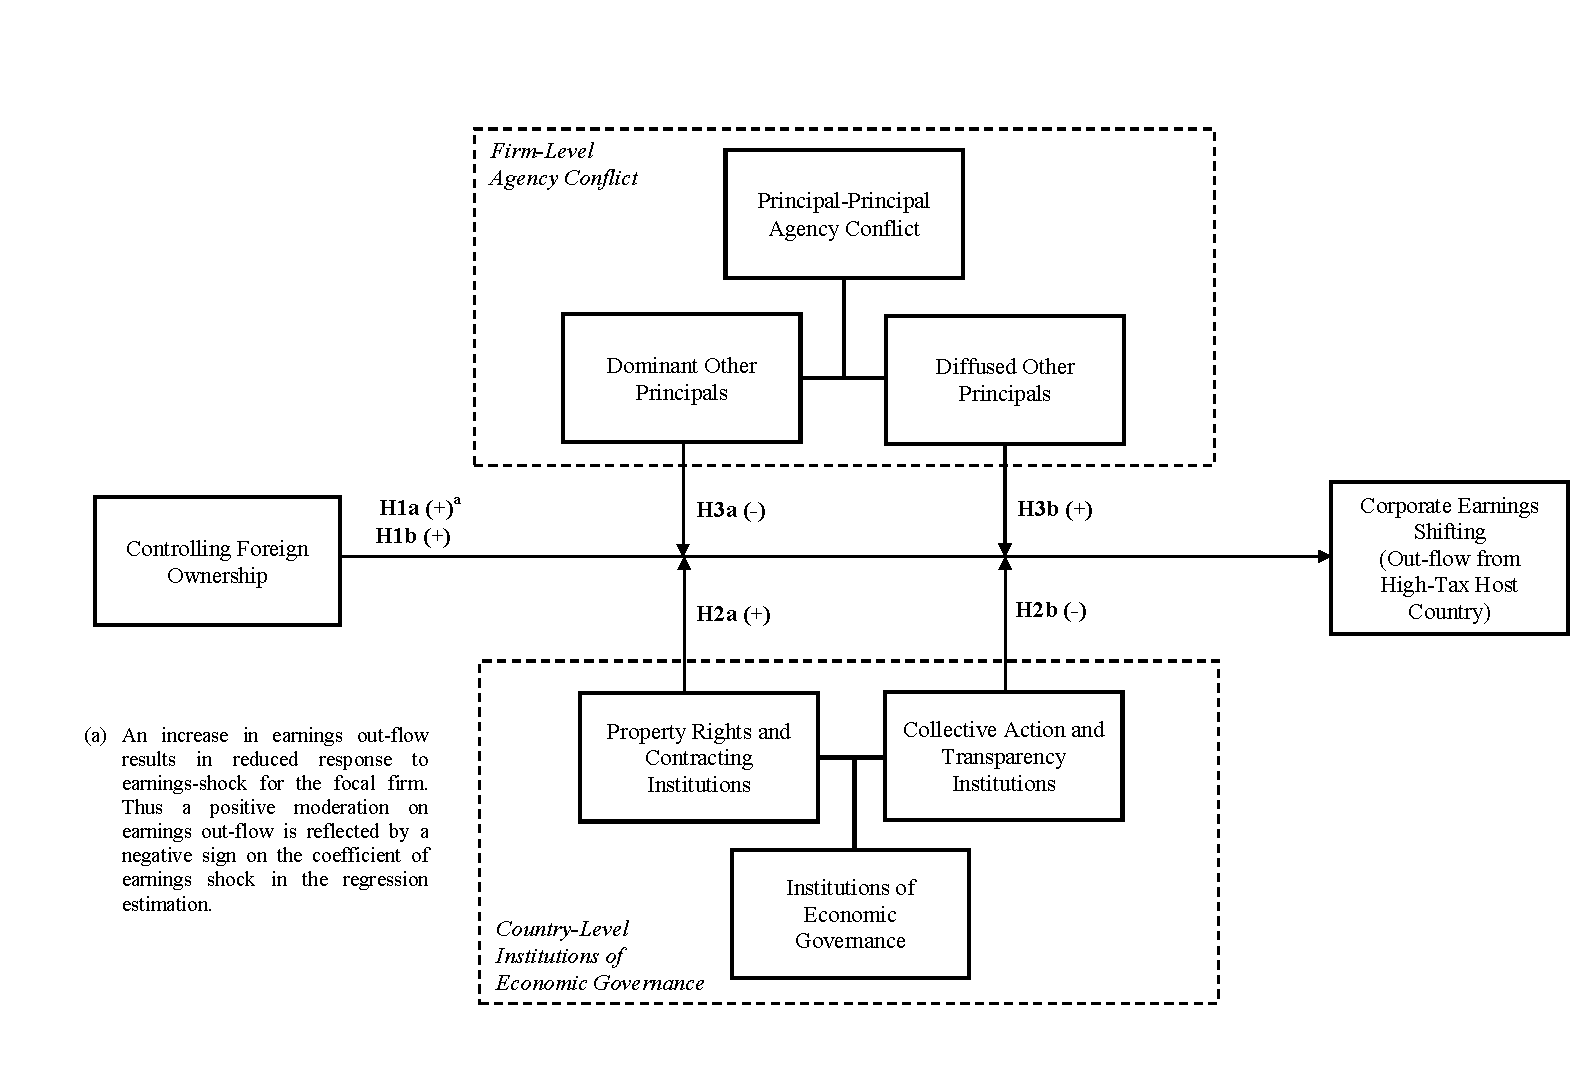
\includegraphics[width=1.00\textwidth]{chapter01/ConceptualModel.pdf}	
\end{sidewaysfigure}

\begin{figure}[h]
	\centering
	\caption{A Simple and Stylized Representation of the Influence of Institutions on the Costs of Extraction of Private Benifits of Control.}
	\vspace{1em}
	\label{fig:costcurve}
	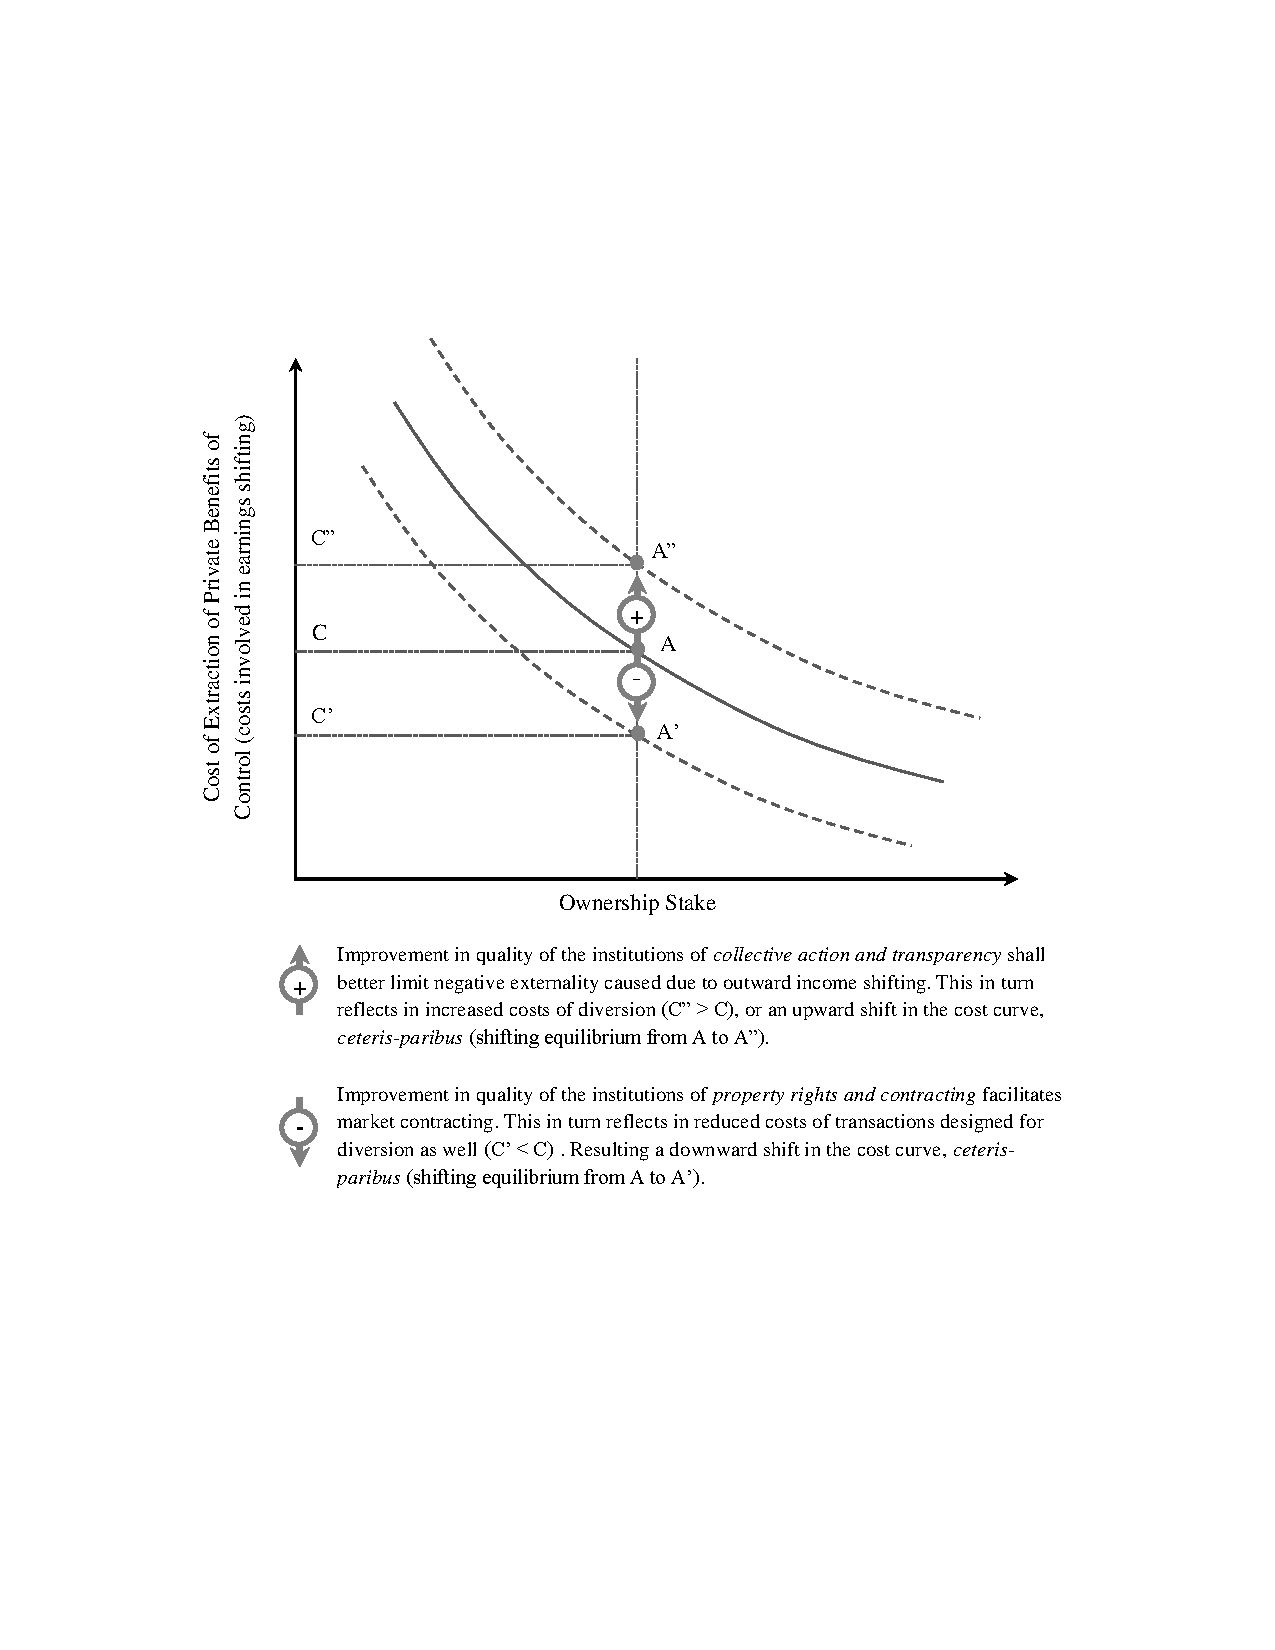
\includegraphics[width=1.00\textwidth]{chapter01/CostCurve.pdf}	
\end{figure}

\begin{figure}[h]
	\centering
	\caption{Temporal Variation in the WGI Measures of Institutional Quality}	
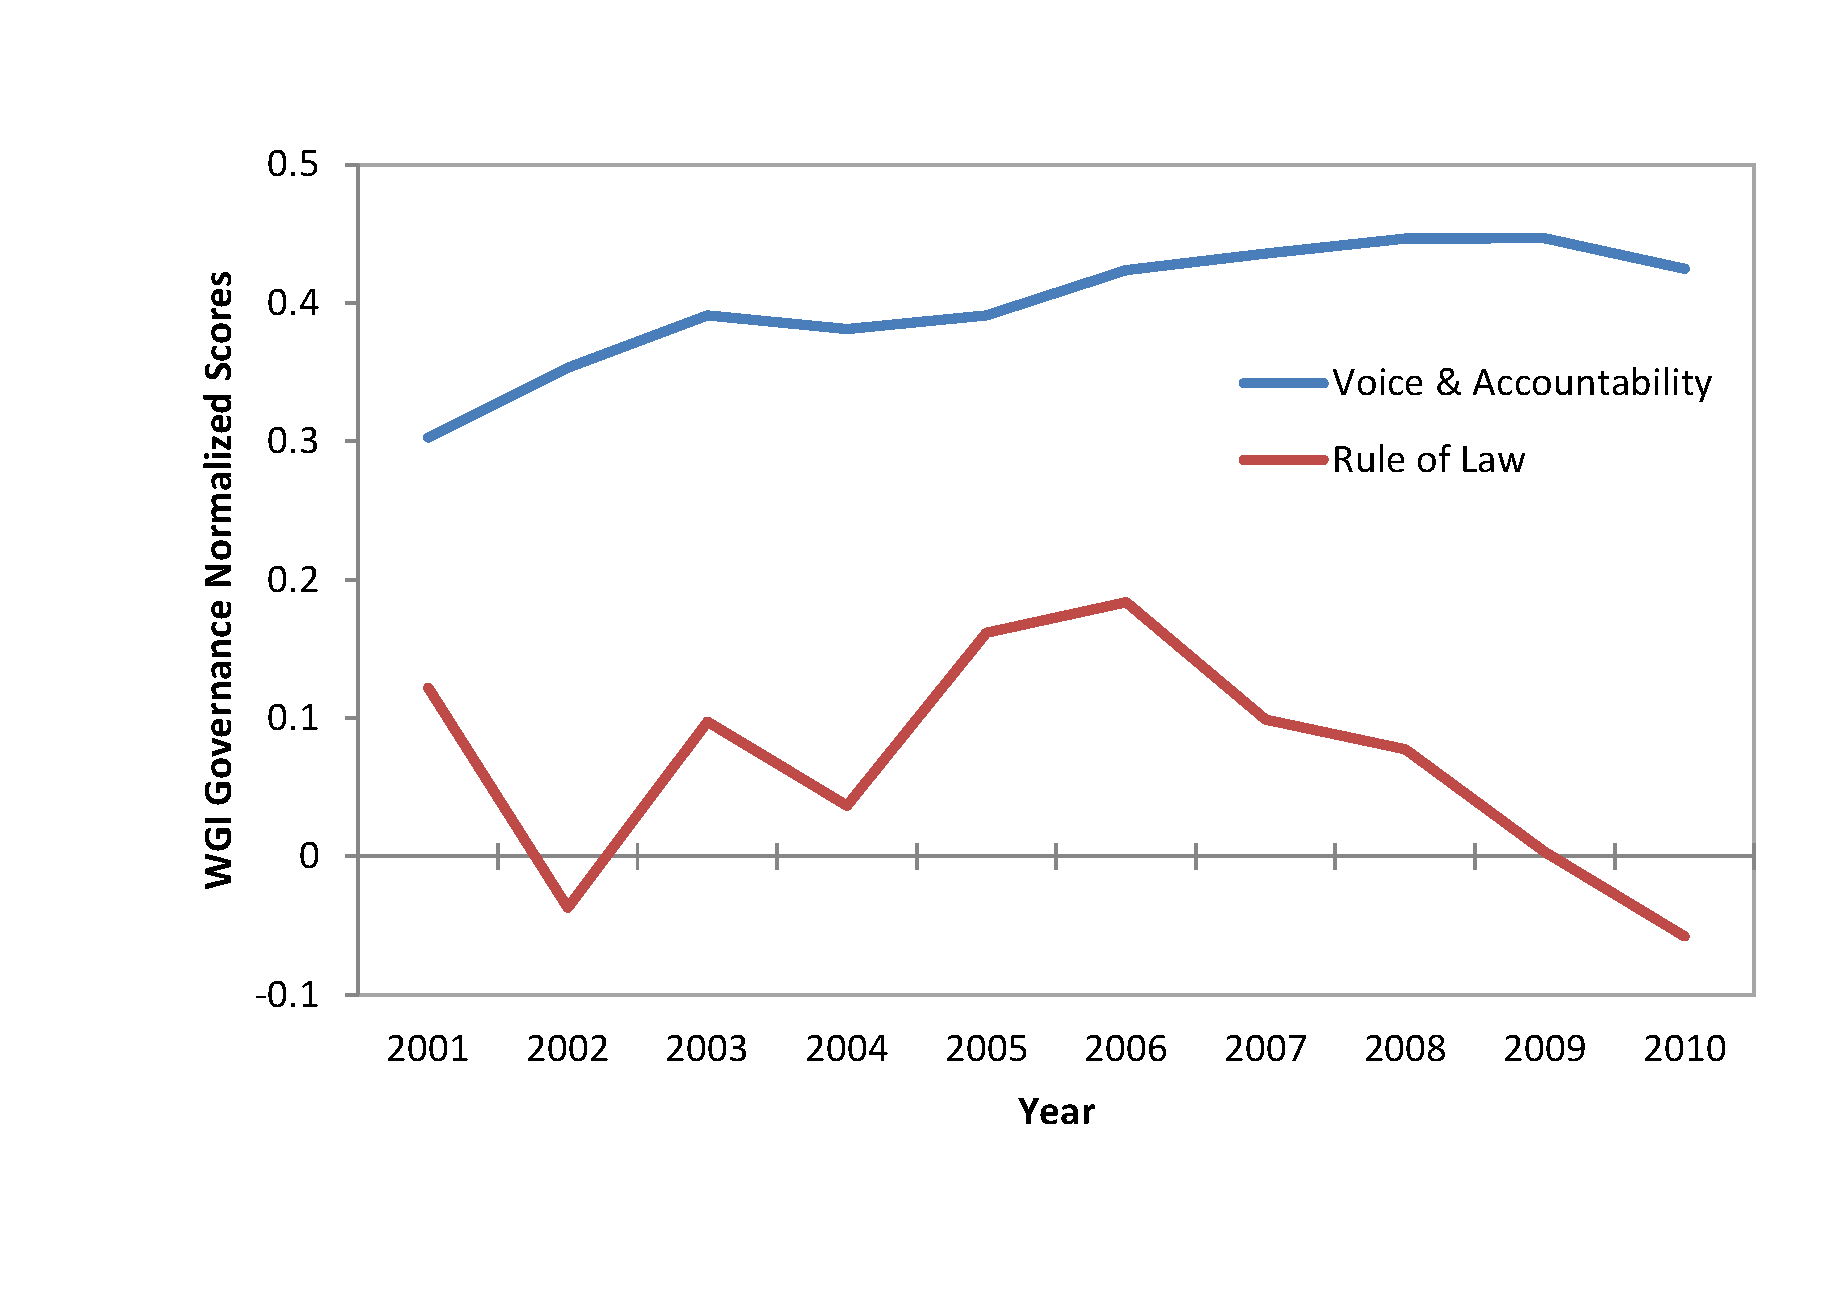
\includegraphics[width=1.00\textwidth]{chapter01/InstitutionalVariations.pdf}
\label{fig:InstitutionalVariations}
\end{figure}


\begin{figure}[h] 
	\centering	
		\caption{Influence of Institutions of Economic Governance on Corporate Earninigs Shifting.}
		\vspace{1em}
	\label{fig:InterInst}
	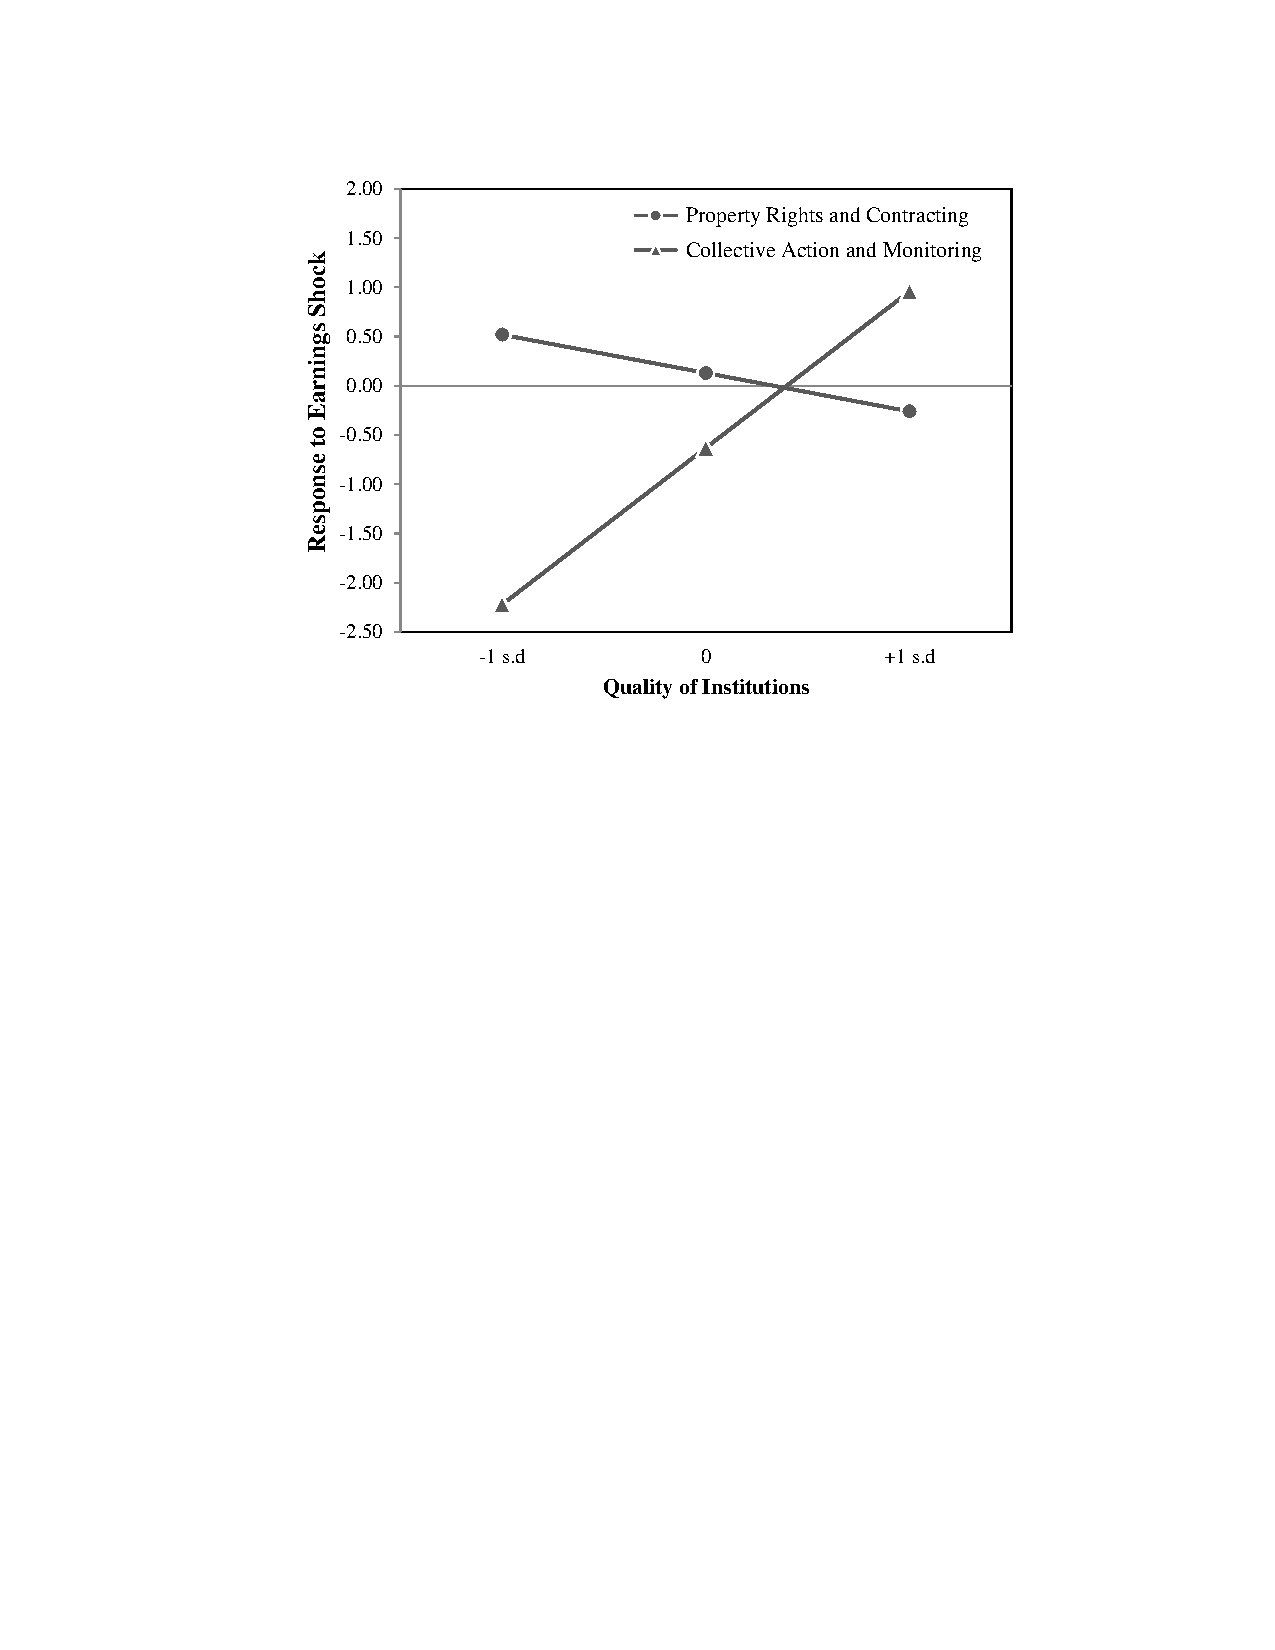
\includegraphics[width=1.00\textwidth]{chapter01/Interactions-PRnC.pdf}		
\end{figure}
\begin{figure}[h]
	\centering
	\caption{Influence of the Principal-Principal Agency Conflict on Earninigs Shifting.}
	\vspace{1em}
	\label{fig:Interppa}
	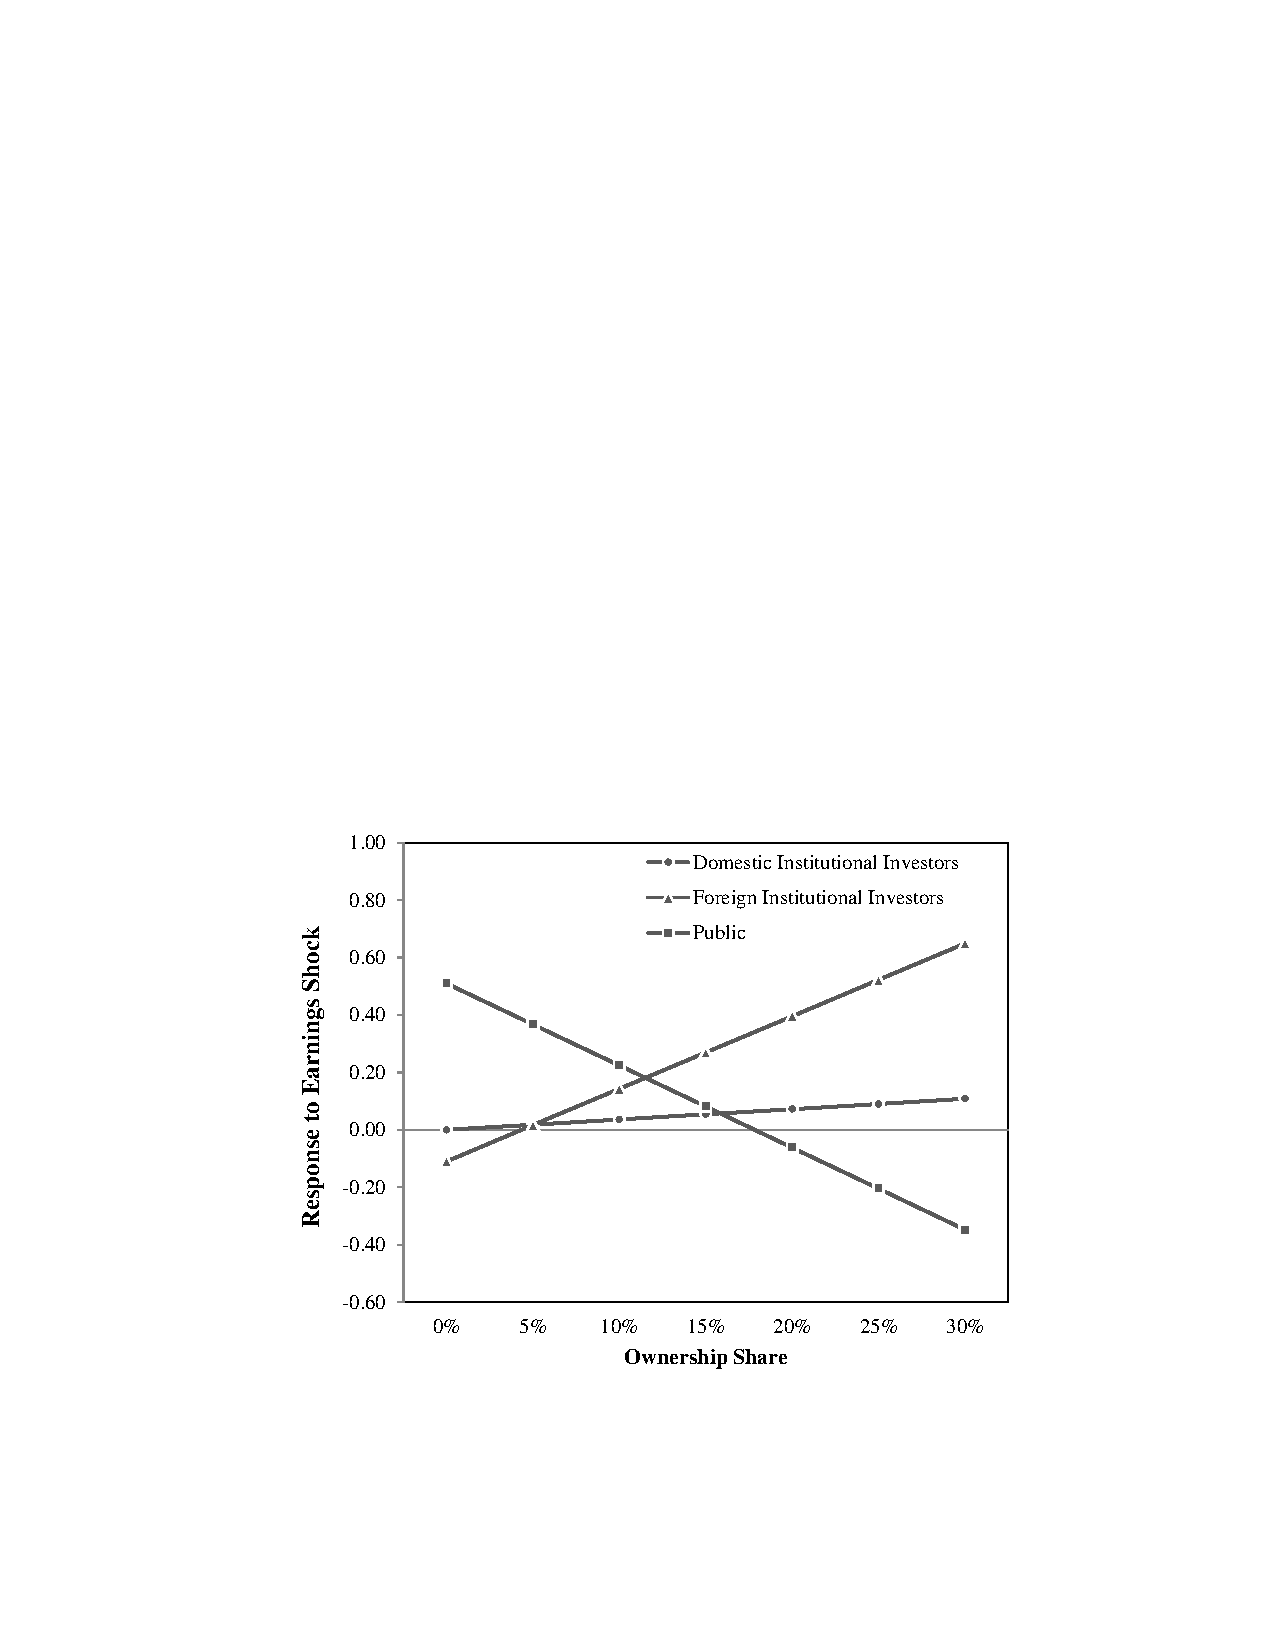
\includegraphics[width=1.00\textwidth]{chapter01/Interactions-PPA.pdf}	
\end{figure}



\bibliographystyle{apalike} 
\newpage
%\singlespacing
\onehalfspacing
\bibliography{chap01refs}
%\doublespacing
%\singlespacing